
%
%  $Description: Author guidelines and sample document in LaTeX 2.09$
%
%  $Author: ienne $
%  $Date: 1995/09/15 15:20:59 $
%  $Revision: 1.4 $
%

\documentclass{sig-alternate}
\usepackage{url}
%\usepackage{times}
%\usepackage{diagrams}
%\usepackage[all]{xy}
\usepackage[ruled,vlined]{algorithm2e}
%\usepackage{float}
\usepackage{times}
\usepackage{graphicx}
\usepackage{epsf}
\usepackage{verbatim}
\usepackage{psfig}
\usepackage{cite}
\usepackage{url}
\usepackage{color}
\usepackage{alltt}

\usepackage{longtable,lscape}
\usepackage{slashbox,multirow}
\usepackage{colortbl}
\usepackage{mathrsfs}

\newcommand{\Add}{\CodeIn{add}}
\newcommand{\AVTree}{\CodeIn{AVTree}}
\newcommand{\Assignment}[3]{$\langle$ \Object{#1}, \Object{#2}, \Object{#3} $\rangle$}
\newcommand{\BinaryTreeRemove}{\CodeIn{BinaryTree\_remove}}
\newcommand{\BinaryTree}{\CodeIn{BinaryTree}}
\newcommand{\Caption}{\caption}
\newcommand{\Char}[1]{`#1'}
\newcommand{\CheckRep}{\CodeIn{checkRep}}
\newcommand{\ClassC}{\CodeIn{C}}
\newcommand{\CodeIn}[1]{{\small\texttt{#1}}}
\newcommand{\CodeOutSize}{\scriptsize}
\newcommand{\Comment}[1]{}
\newcommand{\Ensures}{\CodeIn{ensures}}
\newcommand{\ExtractMax}{\CodeIn{extractMax}}
\newcommand{\FAL}{field-ordering}
\newcommand{\FALs}{field-orderings}
\newcommand{\Fact}{observation}
\newcommand{\Get}{\CodeIn{get}}
\newcommand{\HashSet}{\CodeIn{HashSet}}
\newcommand{\HeapArray}{\CodeIn{HeapArray}}
\newcommand{\Intro}[1]{\emph{#1}}
\newcommand{\Invariant}{\CodeIn{invariant}}
\newcommand{\JUC}{\CodeIn{java.\-util.\-Collections}}
\newcommand{\JUS}{\CodeIn{java.\-util.\-Set}}
\newcommand{\JUTM}{\CodeIn{java.\-util.\-TreeMap}}
\newcommand{\JUTS}{\CodeIn{java.\-util.\-TreeSet}}
\newcommand{\JUV}{\CodeIn{java.\-util.\-Vector}}
\newcommand{\JMLPlusJUnit}{JML+JUnit}
\newcommand{\Korat}{Korat}
\newcommand{\Left}{\CodeIn{left}}
\newcommand{\Lookup}{\CodeIn{lookup}}
\newcommand{\MethM}{\CodeIn{m}}
\newcommand{\Node}[1]{\CodeIn{N}$_#1$}
\newcommand{\Null}{\CodeIn{null}}
\newcommand{\Object}[1]{\CodeIn{o}\ensuremath{_#1}}
\newcommand{\PostM}{\MethM$_{post}$}
\newcommand{\PreM}{\MethM$_{pre}$}
\newcommand{\Put}{\CodeIn{put}}
\newcommand{\Remove}{\CodeIn{remove}}
\newcommand{\RepOk}{\CodeIn{repOk}}
\newcommand{\Requires}{\CodeIn{requires}}
\newcommand{\Reverse}{\CodeIn{reverse}}
\newcommand{\Right}{\CodeIn{right}}
\newcommand{\Root}{\CodeIn{root}}
\newcommand{\Set}{\CodeIn{set}}
\newcommand{\State}[1]{2^{#1}}
\newcommand{\TestEra}{TestEra}
\newcommand{\TreeMap}{\CodeIn{TreeMap}}

\newenvironment{CodeOut}{\begin{scriptsize}}{\end{scriptsize}}
\newenvironment{SmallOut}{\begin{small}}{\end{small}}

\newcommand{\pairwiseEquals}{PairwiseEquals}
\newcommand{\monitorEquals}{MonitorEquals}
%\newcommand{\monitorWField}{WholeStateW}
\newcommand{\traverseField}{WholeState}
\newcommand{\monitorSMSeq}{ModifyingSeq}
\newcommand{\monitorSeq}{WholeSeq}

\newcommand{\IntStack}{\CodeIn{IntStack}}
\newcommand{\UBStack}{\CodeIn{UBStack}}
\newcommand{\BSet}{\CodeIn{BSet}}
\newcommand{\BBag}{\CodeIn{BBag}}
\newcommand{\ShoppingCart}{\CodeIn{ShoppingCart}}
\newcommand{\BankAccount}{\CodeIn{BankAccount}}
\newcommand{\BinarySearchTree}{\CodeIn{BinarySearchTree}}
\newcommand{\LinkedList}{\CodeIn{LinkedList}}

\newcommand{\Book}{\CodeIn{Book}}
\newcommand{\Library}{\CodeIn{Library}}

\newcommand{\Jtest}{Jtest}
\newcommand{\JCrasher}{JCrasher}
\newcommand{\Daikon}{Daikon}
\newcommand{\JUnit}{JUnit}

\newcommand{\trie}{trie}

\newcommand{\Perl}{Perl}


\newcommand{\SubjectCount}{11}
\newcommand{\DSSubjectCount}{two}

\newcommand{\Equals}{\CodeIn{equals}}
\newcommand{\Pairwise}{PairwiseEquals}
\newcommand{\Subgraph}{MonitorEquals}
\newcommand{\Concrete}{WholeState}
\newcommand{\ModSeq}{ModifyingSeq}
\newcommand{\Seq}{WholeSeq}
\newcommand{\Aeq}{equality}

\newcommand{\Meaning}[1]{\ensuremath{[\![}#1\ensuremath{]\!]}}
\newcommand{\Pair}[2]{\ensuremath{\langle #1, #2 \rangle}}
\newcommand{\Triple}[3]{\ensuremath{\langle #1, #2, #3 \rangle}}
\newcommand{\SetSuch}[2]{\ensuremath{\{ #1 | #2 \}}}

\newcommand{\Equiv}[2]{\ensuremath{#1 \EquivSTRel{} #2}}
\newcommand{\EquivME}{\Equiv}
\newcommand{\EquivST}{\Equiv}
\newcommand{\EquivSTRel}{\ensuremath{\cong}}
\newcommand{\Redundant}[2]{\ensuremath{#1 \lhd #2}}
\newcommand{\VB}{\ensuremath{\mid}}
\newcommand{\MES}{method-entry state}

\newcommand{\Small}[1]{{\small{#1}}}

\newcommand{\CenterCell}[1]{\multicolumn{1}{c|}{#1}}

%\documentstyle[times,art10,twocolumn,latex8]{article}

%-------------------------------------------------------------------------
% take the % away on next line to produce the final camera-ready version
\pagestyle{empty}

%-------------------------------------------------------------------------
\begin{document}

\conferenceinfo{ICSE}{'11, May 21-28 2011, Waikiki, Honolulu, Hawaii}
\CopyrightYear{2011}
%\crdata{978-1-60558-719-6/10/05}


\title{Automated Testing of API Mapping Relations}

%\author{
%Hao Zhong$^{1,2}$\thanks{Corresponding authors}, Suresh Thummalapenta$^4$, Tao Xie$^{4*}$\\
%\small{$^1$Laboratory for Internet Software Technologies, Institute of Software, Chinese Academy of Sciences, Beijing, 100190, China}\\
%\small{$^2$Key Laboratory of High Confidence Software Technologies (Peking University), Ministry of Education, China}\\
%\small{$^3$Institute of Software, School of Electronics Engineering and Computer Science, Peking University, China} \\
%\small{$^4$Department of Computer Science, North Carolina State University, Raleigh, NC 27695-8206, USA}\\
%\small{zhonghao@itechs.iscas.ac.cn, \{sthumma,txie\}@ncsu.edu}}
\numberofauthors{2}
\author{
% You can go ahead and credit any number of authors here,
% e.g. one 'row of three' or two rows (consisting of one row of three
% and a second row of one, two or three).
%
% The command \alignauthor (no curly braces needed) should
% precede each author name, affiliation/snail-mail address and
% e-mail address. Additionally, tag each line of
% affiliation/address with \affaddr, and tag the
% e-mail address with \email.
%
% 1st. author
\alignauthor
Hao Zhong\\
       \affaddr{Laboratory for Internet Software Technologies}\\
       \affaddr{Institute of Software}\\
       \affaddr{Chinese Academy of Sciences, China}\\
       \email{zhonghao@nfs.iscas.ac.cn}
% 2nd. author
\alignauthor
Suresh Thummalapenta and Tao Xie\\
       \affaddr{Department of Computer Science}\\
       \affaddr{North Carolina State University}\\
       \affaddr{Raleigh, NC 27695-8206, USA}\\
       \email{\{sthumma,txie\}@ncsu.edu}
}
\maketitle
\thispagestyle{empty}

\begin{abstract}

Software companies or open source organizations often release their applications in different languages to address business requirements such as platform independence. To produce the same applications in different languages, existing applications already in one language such as Java are translated to applications in a different language such as C\#. To translate applications from one language ($L_1$) to another language ($L_2$), programmers often use automatic translation tools. These translation tools use Application Programming Interface (API) mapping relations from $L_1$ to $L_2$ as a basis for translation. It is essential that API elements (\emph{i.e.}, classes, methods, and fields) of $L_1$ and their mapped API elements of $L_2$ (as described by API mapping relations) exhibit the same behavior, since any inconsistencies among these mapping relations could result in behavioral differences and defects in translated applications. Therefore, to detect behavioral differences between mapped API elements described in mapping relations, and thereby to effectively translate applications, we propose the first novel approach, called \emph{TeMAPI} (\textbf{Te}sting \textbf{M}apping relations of \textbf{API}s). In particular, given a translation tool, TeMAPI automatically generates test cases that expose behavioral differences between mapped API elements from mapping relations described in the tool. To show the effectiveness of our approach, we applied our approach on five popular translation tools. The results show that TeMAPI effectively detects various behavioral differences between mapped API elements. We summarize detected differences as eight findings and their implications. Our approach enables us to produce these findings that can improve effectiveness of translation tools, and also assist programmers in understanding the differences between mapped API elements of different languages.
\end{abstract}\vspace*{-2ex} %% A category with the (minimum) three required fields
%\category{D.2.13 Reusable Software}{Reusable Software}{Reusable libraries}\vspace*{-2ex}
%%A category including the fourth, optional field follows...
%\terms{API mapping relation, Language migration}\vspace*{-2ex}

\section{Introduction}
\label{sec:introduction}

Since the inception of computer science, many programming languages (\emph{e.g.}, Cobol, Fortran, or Java) have been introduced to serve specific requirements\footnote{\url{http://hopl.murdoch.edu.au}}. For example, Cobol is introduced specifically for developing business applications. In general, software companies or open source organizations often release their applications in different languages to survive in competing markets and to address various business requirements such as platform independence. An empirical study~\citep{jones1998estimating} shows that nearly one third applications have multiple versions in different languages. A natural way to implement an application in a different language is to translate from an existing application. For example, Lucene.Net was translated from Java Lucene according to its website\footnote{\url{http://lucene.apache.org/lucene.net/}}. As another example, the NeoDatis object database was also translated form Java to C\# according to its website\footnote{\url{http://wiki.neodatis.org/}}. During translation, one primary goal is to ensure that both applications exhibit the same behavior.

As existing applications typically use API libraries, it is essential to understand API mapping relations of one programming language, referred to as $L_1$, to another language, referred to as $L_2$, when translating applications from $L_1$ to $L_2$. Researchers~\citep{robillard2009makes,thomas2006api} pointed out that it is hard to use API elements, and our previous work~\citep{zhong2010mining} shows that mapping relations between API elements of different languages can also be complicated. In some cases, programmers may fail to find an existing API element that has the same behavior in the other language. For example, Figures~\ref{fig:db4ojava} and \ref{fig:db40net} show two methods implemented in db4o\footnote{\url{http://www.db4o.com}} of its Java version and its C\# version, respectively. When translating the Java code shown in Figure~\ref{fig:db4ojava} to C\#, programmers of db4o may fail to find an existing C\# class that has the same behaviors with the \CodeIn{Byte\-Array\-Input\-Stream} class in Java, so they implement a C\# class with the same name to fix the behavioral difference. Behavioral differences of mapped API elements (\emph{i.e}., classes, methods, and fields of API libraries) may occur in many places. To reduce translation effort, programmers of db4o developed their own translation tool, called Sharpen\footnote{\url{http://developer.db4o.com/Blogs/News/tabid/171/entryid/653/Default.aspx}}, for translating db4o from Java to C\#. For API translation, Sharpen systematically replaces all API elements in Java with equivalent elements in C\# to ensure that translated C\# applications have the same behaviors with the original Java ones.

\begin{figure}[t]
\begin{CodeOut}%\vspace*{-2ex}
\begin{alltt}
01: private long readLong(ByteArrayInputStream is)\{
02:  ...
03:  l += ((long) (is.read())) << i;
04:  ...\}
\end{alltt}
\end{CodeOut}%\vspace*{-4ex}
\caption{A method in the Java version of db4o.}%\vspace*{-2ex}
\label{fig:db4ojava}
\begin{CodeOut}%\vspace*{-2ex}
\begin{alltt}
05: private long ReadLong(ByteArrayInputStream @is)\{
06:  ...
07:  l += ((long)(@is.Read())) << i;
08:  ...\}
\end{alltt}
\end{CodeOut}%\vspace*{-4ex}
\caption{A method in the C\# version of db4o.}%\vspace*{-4ex}
\label{fig:db40net}
\end{figure}

In practice, as pointed out by Keyvan Nayyeri\footnote{\url{http://dotnet.dzone.com/print/26587}}, one of the most common problems is that translated code does not return expected outputs, partially because behavioral differences of mapped API elements are not fully fixed. For example, when JLCA\footnote{JLCA is a Java-to-C\# translation tool developed by Microsoft. The website of JLCA is \url{http://msdn.microsoft.com/en-us/magazine/cc163422.aspx}} translates the \CodeIn{java.lang.String.indexOf(int)} method from Java to C\#, it generates a warning message: ``Method \CodeIn{java.lang.String. indexOf} was converted to \CodeIn{System.String.IndexOf}, which may throw an exception''. Still, the report does not describe where such an exception is thrown or how to deal with that exception. As programmers typically do not know where such behavioral differences occur, it is difficult for programmers to fix such differences in advance, and thus defects can be introduced in translated applications. To prevent those defects, it is desirable to detect behavioral differences between mapped API elements in different languages. However, existing approaches~\citep{orso1using,jin2010automated,jiang2009automatic,lindigaadebug2005} solve different problems, and cannot detect such differences effectively since these existing approaches require that both the versions under consideration belong to the same language. In our context, the versions under consideration belong to different languages, making these existing approaches inapplicable.


To address the preceding issue, we propose a novel approach, called TeMAPI (\textbf{Te}sting \textbf{Ma}pping relations of \textbf{API}s), that generates test cases to detect behavioral differences among API mapping relations automatically. In particular, TeMAPI accepts two inputs: a translation tool under analysis and a test-generation tool for generating test cases. Given a translation tool that translates applications from one language $L_1$ to the other language $L_2$, TeMAPI generates various test cases to detect behavioral differences among the API mapping relations by effectively leveraging the test-generation tool. TeMAPI next executes translated test cases to detect behavioral differences.

TeMAPI addresses four major technical challenges in effectively detecting behavioral differences. (1) It is challenging to directly extract API mapping relations from translation tools. The primary reason is that often translation tools either use different formats for specifying API mapping relations or do not explicitly describe these mapping relations. For example, Java2CSharp\footnote{Java2CSharp is a Java-to-C\# translation tool developed by ILOG (now IBM). The website of Java2CSharp is \url{http://j2cstranslator.sourceforge.net/}} uses mapping files, Sharpen hardcodes relations in source files, and closed source translation tools such as JLCA typically hide mapping relations in binary files. To address this issue and to be independent of the translation tool under analysis, TeMAPI analyzes translated code for extracting those relations. (2) Interfaces of two mapped API elements can be different, and one API element can be translated to multiple API elements. For example, JLCA translates the \CodeIn{java.net.DatagramSocket.receive(DatagramPacket)} method in Java as shown in Figure~\ref{fig:javacode} to multiple C\# elements as shown in Figure~\ref{fig:codeJLCA}.
To address this issue, TeMAPI uses a technique, called wrapper methods (Section~\ref{sec:approach:wrapper}), that abstracts interface differences among mapped API elements and provides a common interface to effectively apply test-generation tools. (3) Using a basic technique such as generating test cases with \CodeIn{null} values may not be significant in detecting behavioral differences among API mapping relations. Since we focus on object-oriented languages such as Java or C\# to detect behavioral differences, generated test cases need to exercise various object states, which can be achieved using method-call sequences. To address this issue, TeMAPI leverages two existing state-of-the-art test-generation techniques: random~\citep{pacheco2007feedback} and dynamic-symbolic-execution-based~\citep{koushik:cute, godefroid:dart, tillmann2008pex} ones. (4) API elements are typically quite large in size, and it is difficult to check all outputs, posing a test oracle barrier. To overcome the barrier, TeMAPI uses return values of wrapper methods or exceptions being thrown as test oracles. We describe more details of our approach to address these challenges in subsequent sections.

In this paper, although we present our approach for detecting behavioral differences among mapping relations of different languages, our approach is general and can be applied to other software engineering problems where an API needs to be replaced with another API without changing the behavior of an application (\emph{e.g.}, library upgrades~\citep{Kawrykow:2009} or migrating from one library to another library~\citep{nita2010using}).

This paper makes the following major contributions:

\begin{itemize}\vspace*{-1ex}
\item A novel approach, called TeMAPI, that automatically generates test cases to detect behavioral differences among API mapping relations. %\vspace*{-1.5ex}
\item A tool implemented for TeMAPI and four evaluations on five popular translation tools. Unlike untranslated code elements, behavioral differences introduce no compilation errors to be detected, and can lead to defects in translated applications silently. Our results show that existing translation tools can translate most lines from Java to C\#, although these tools typically cover a small set of API mapping relations. Our results also show the effectiveness of our approach in detecting behavioral differences of mapped API elements between different languages.
\item The first empirical comparison on behavioral differences of mapped API elements between the J2SE and .NET frameworks. As shown in Section~\ref{sec:evaluation}, the comparison reveals 8 behavioral differences between mapped API elements in existing translation tools. We analyze these findings, and conclude their implications that are valuable to vendors of translation tools for improving their tools, programmers who use translation tools for being aware of such differences in advance, and developers of API libraries for implementing more translatable APIs.
\end{itemize}\vspace*{-1ex}

The rest of this paper is organized as follows.
%Section~\ref{sec:mapping} presents our test adequacy criteria.
Section~\ref{sec:example} presents an illustrative example.
Section~\ref{sec:approach} presents our approach.
Section~\ref{sec:evaluation} presents our evaluation.
Section~\ref{sec:real} presents capabilities of existing translation tools to translate real projects and discusses importance of our major findings.
Section~\ref{sec:discuss} discusses issues of our approach.
Section~\ref{sec:related} presents related work.
Section~\ref{sec:conclusion} concludes.
\begin{figure}[t]
\begin{CodeOut}%\vspace*{-2ex}
\begin{alltt}
09: DatagramSocket socket = ...;
10: DatagramPacket package = ...;
11: socket.receive(package);
\end{alltt}
\end{CodeOut}%\vspace*{-5ex}
\caption{Sample code in Java.}%\vspace*{-2ex}
\label{fig:javacode}
\begin{CodeOut}%\vspace*{-2ex}
\begin{alltt}
12: UdpClient socket = ...;
13: IPEndPoint remoteIpEndPoint = ...;
14: try\{
15:  byte[] data_in = socket.Receive(ref remoteIpEndPoint);
16:  PacketSupport tempPacket =
          new PacketSupport(data_in, data_in.Length);
17:   tempPacket.IPEndPoint = remoteIpEndPoint;
18: \} catch (System.Exception e)\{...\}
19: PacketSupport package = tempPacket;
\end{alltt}
\end{CodeOut}%\vspace*{-5ex}
\caption{Translated C\# code by JLCA.}%\vspace*{-4ex}
\label{fig:codeJLCA}
\end{figure}

%As stated by Sebesta~\citep{sebesta2002concepts}, modern programming languages start around 1958 to 1960 with the development of Algol, Cobol, Fortran and Lisp. Ever since then, thousands of programming languages came to existence as shown by HOPL website\footnote{\url{http://hopl.murdoch.edu.au}}. For various considerations, programmers often need to translate projects from one language to another language. For example, as stated by , to provide the language and platform independence, he translates Compose*~\citep{garcia-compose} in C\# to Compose*/J in Java. To relief the efforts of translating, programmers may use existing translation tools or even implement their own translation tools. For example, Salem \emph{et al.}~\citep{AgtashAEMBS06} report their experience of translating the BLUE financial system of the ICT company from Java to C\# by the JLCA\footnote{\url{http://tinyurl.com/2c4coln}} tool. For another example, to translate db4o\footnote{\url{http://www.db4o.com}} from Java to C\#, its programmers develop their own translation tool named Sharpen\footnote{\url{http://tinyurl.com/22rsnsk}}.

%To translate a source file, a translation tool needs to its structures and its used API elements. As a project typically use thousands of API elements, it is often more difficult to translate used API elements especially for those languages whose structures are similar. In particular, El-Ramly \emph{et al.}~\citep{el2006experiment} conduct an experiment to translate Java programs to C\#. One of their learnt lessons is ``it
%becomes very important to develop methods for
%automatic API transformation''. Barry compares C\# with Java\footnote{\url{http://tinyurl.com/26d8xcp}}, and claims ``although coding in C\# is easy for a Java programmer..., the biggest challenge in moving from Java to the .NET Framework is learning the details of another set of class libraries''. If not knowing API mapping relations, a translation tool or a programmer cannot translate used API elements correctly. Even when such mapping relations are available, a migration process may introduce defects in translated code since mapped API elements can have behavioral differences. As reported by Panesar\footnote{\url{http://tinyurl.com/3xpsdtx}}, even most common methods such as \CodeIn{String.subString(int, int)} can have behavioral differences between Java and C\#. We investigate the mapping relations of existing translation tools, and we confirm that the behavioral differences of mapped API elements can cause defects in translated code. In particular, in Java2CSharp\footnote{\url{http://j2cstranslator.sourceforge.net/}}, one item of mapping files is described in its mapping files as follows:
%
%\begin{CodeOut}%\vspace*{-2ex}
%\begin{alltt}
%1 package java.lang::System\{
%2  class java.lang.String :: System:String\{
%3   method valueOf(Object) { pattern = @1.ToString(); }
%4   ...\}\}
%\end{alltt}
%\end{CodeOut}
%
%Line 2 of this item describes that the \CodeIn{java.lang.String} class in Java is mapped to the \CodeIn{System.String} class in C\#. Line 3 of this item describes that the \CodeIn{java.lang.String.valueOf(Object)} method is mapped to the \CodeIn{System.String.ToString()} method in C\#, and \CodeIn{@1} denotes the first parameter of the \CodeIn{valueOf(Object)} method. Based on the preceding mapping relation, Java2CSharp translates a Java code snippet (Lines 5 and 6) to a C\# code snippet (Lines 7 and 8) as follows.
%
%\begin{CodeOut}%\vspace*{-2ex}
%\begin{alltt}
%\textbf{  Java Code}
%5 Object obj = ...
%6 String value = java.lang.String.valueOf(obj);
%\textbf{  C# Code translated by Java2CSharp}
%7 Object obj = ...
%8 String value = obj.ToString();
%\end{alltt}
%\end{CodeOut}
%
%The translated code snippet compile well, but it has behavioral differences with the original Java code snippet. For example, if Line 5 assigns null to \CodeIn{obj}, \CodeIn{value} of Line 6 will be ``null''. If Line 7 assigns null to \CodeIn{obj}, \CodeIn{value} of Line 8 will not be set to ``null'' since it throws \CodeIn{NullReferenceException}.
%
%As it throw exceptions, the preceding difference of API mapping relation is relatively easy to detect since programmers often use extreme inputs such as null values as test cases. In particular, Sharpen is aware of the differences, and the mapping relation in Sharpen is defined as follows:
%
%\begin{CodeOut}
%\begin{alltt}
%9 public abstract class Configuration \{
%10 protected void setUpStringMappings() \{
%11   mapMethod("java.lang.String.valueOf",
%              runtimeMethod("getStringValueOf"));
%12  ...\} \}
%\end{alltt}
%\end{CodeOut}
%
%Based on Line 11 of the preceding mapping relation, Sharpen translates the Java code snippet (Lines 5 and 6) to a C\# code snippet (Lines 7 and 8) as follows.
%
%\begin{CodeOut}%\vspace*{-2ex}
%\begin{alltt}
%\textbf{  C# Code translated by Sharpen}
%13 Object obj = ...
%14 String value = getStringValueOf(obj);
%\end{alltt}
%\end{CodeOut}
%
%In Sharpen, the \CodeIn{getStringValueOf(object)} method is implemented as follows:
%
%\begin{CodeOut}%\vspace*{-2ex}
%\begin{alltt}
%15 public static string GetStringValueOf(object value)\{
%16  return null == value? "null": value.ToString();
%17	\}
%\end{alltt}
%\end{CodeOut}
%
%If Line 13 assigns a null value to \CodeIn{obj}, \CodeIn{value} in Line 14 will also be ``null'' as expected. By implementing its own mapped C\# method, Sharpen hides the preceding difference, but it still fails to hide all differences. For example, we find that if Line 5 assigns a \CodeIn{false} boolean value to \CodeIn{obj}, \CodeIn{value} in Line 6 will be ``false'', but if Lines 7 and 13 assign a \CodeIn{false} boolean value to \CodeIn{obj}, \CodeIn{value} of Line 8 and \CodeIn{value} in Line 14 will both be ``False''. This difference is relatively difficult to detect, since a programmer typically does not know the internal logic of the method to construct appropriate test cases.
%
%
%It is desirable to detect differences of API mapping relations since the differences will potentially introduce defects to client codek, the same inputs, but it is challenging to detect behavioral differences of API mapping relations via testing for three factors: (1) API elements are typically quite large in size, so it takes great efforts to write test cases manually for API elements and their mapping relations; (2) Other types of migrations such as library migrations~\citep{nita2010using} can use existing test cases to ensure the quality of migrated code, but for language migration, translated test cases may also have defects at the first place; (3) It requires many test cases to reveal all behaviors of API elements, and simply generating extreme values such as null values are not sufficient to reveal all API behaviors.
%
%In this paper, we propose an approach, called TeMAPI (\textbf{Te}sting \textbf{Ma}pping relations of \textbf{API}s), that detects behavioral differences of API mapping relations via testing. TeMAPI generates various test cases and compares testing results of mapped API elements for their behavioral differences. This paper makes the following major contributions:
%
%\begin{itemize}\vspace*{-1.5ex}
%\item A novel approach, called TeMAPI, that detect behavioral differences of mapped API elements via testing. Given a translation tool, TeMAPI detects behavioral differences of its all API mapping relations automatically. It is important to detect these behavioral differences since they can introduce defects in translated code silently.\vspace*{-1.5ex}
%\item Test adequacy criteria proposed for generating sufficient test cases to test API mapping. TeMAPI targets at generating adequate test cases that can reveal all behaviors of API elements to test their mapping relations.\vspace*{-1.5ex}
%\item A tool implemented for TeMAPI and two
%evaluations on ?? projects that include ?? mapping relations from Java to C\#, and ?? mapping relations from C\# to Java. The results show that our tool detects ?? unique defects of mapping relations...
%\end{itemize}\vspace*{-1.5ex}
%
%The rest of this paper is organized as follows.
%Section~\ref{sec:mapping} presents our test adequacy criteria.
%Section~\ref{sec:example} illustrates our approach using an example.
%Section~\ref{sec:approach} presents our approach.
%Section~\ref{sec:evaluation} presents our evaluation results.
%Section~\ref{sec:discuss} discusses issues of our approach.
%Section~\ref{sec:related} presents related work.
%Finally, Section~\ref{sec:conclusion} concludes.

%\section{Background}
\label{sec:background}

We next provide details of two major concepts used in the rest of
the paper: dynamic symbolic execution and dynamic code coverage.

%-----------------------------------------------------------------------------
\subsection{Dynamic Symbolic Execution}

In our approach, we use Pex as an example state-of-the-art dynamic symbolic 
execution tool. Pex~\cite{tillman:pexwhite} is an automatic unit-test-generation 
tool developed by Microsoft. Pex accepts PUTs as input and generates conventional 
unit tests that can achieve high 
structural coverage of the code under test. Initially, Pex
executes the code under test with random inputs. While executing
the code under test, Pex collects constraints on inputs from predicates
in branching statements. Pex next solves collected constraints
to generate new test inputs that guide future executions along
new paths. Pex includes various optimization techniques such as
reducing the size of the formula before giving it over constraint solver.

%-----------------------------------------------------------------------------
\subsection{Dynamic Code Coverage}

In this paper, we use Pex generated reports for measuring coverage. These coverage
reports are called dynamic, because Pex knows only about the code that was already executed.
As Pex is not aware of the code that is not yet executed, dynamic code coverage
cannot give absolute values for the coverage. The primary reason for using
dynamic code coverage in our paper is that C\# allows generate code during run time.
Therefore, it is often not possible to find out how much code exists beforehand.
%\section{Definitions}
\label{sec:mapping}

We next present definitions of terms used in the rest of the paper.

\textbf{API:} An Application Programming Interface (API)~\cite{orenstein2000quickstudy}
is a set of classes and methods provided by frameworks or libraries.

\textbf{API library:} An API library refers to a framework
or library that provides reusable API classes and methods.

\textbf{Client code:} Client code refers to the application code
that reuses or extends API classes and methods provided by API
libraries. The definitions of API library and client code are
relative to each other. For example, Lucene uses
J2SE\footnote{\url{http://java.sun.com/j2se/1.5.0/}} as an API
library, whereas Nutch\footnote{\url{http://lucene.apache.org/nutch/}} uses Lucene as
an API library. Therefore, we consider Lucene as client code and API
library for the J2SE API library and Nutch, respectively. In
general, for client code, source files of API libraries are often
not available.

\textbf{Mapping relation:} A mapping relation refers to a
replaceable relation among entities such as API classes or methods
defined by two different languages. For example, consider two
languages $L_1$ and $L_2$, and two entities $e_1$ and $e_2$ in
$L_1$ and $L_2$, respectively. We define a mapping
relation between $e_1$ and $e_2$, if $e_1$ of $L_1$ can be translated to $e_2$ of $L_2$
without introducing new defects in the translated code.

\textbf{Mapping relation of API classes:} We define a mapping
relation between two API classes $c_1$ and $c_2$ of $L_1$ and $L_2$,
respectively, if $c_1$ of $L_1$ is translated to $c_2$ of $L_2$
without introducing new defects in the translated code.

Our mapping relation of API classes is many-to-many. For example,
\CodeIn{java.util.ArrayList} of Java is mapped to either
\CodeIn{System. Collections.ArrayList} \textbf{or}
\CodeIn{System.Collections.Generic. List} of C\#, whereas
\CodeIn{java.lang.System} of Java is mapped to
\CodeIn{System.DataTime} \textbf{and} \CodeIn{System.Environment} of
C\# based on how client code uses these classes. In particular, when
client code uses APIs to get the current time,
\CodeIn{java.lang.System} is mapped to \CodeIn{System.DataTime}. In
contrast, when client code uses APIs to get environment settings,
\CodeIn{java.lang.System} is mapped with
\CodeIn{System.Environment}.

Furthermore, mapped API classes may have different behaviors. For
example, \CodeIn{java.lang.String} of Java is mapped to
\CodeIn{System. String} of C\#. However, \CodeIn{System.String} has
an API method \CodeIn{insert}, which does not exist in
\CodeIn{java.lang.String}.

\textbf{Mapping relation of API methods:} We define a mapping relation
between two API methods $m_1$ and $m_2$ of languages $L_1$ and $L_2$,
respectively, if $m_1$ is translated to $m_2$ without introducing defects
in the translated code.

\textbf{Merged API method:} A merged API method of $L_1$ refers to
an API method that is created by merging two other API methods of
$L_1$. For example, consider two API methods $m_1$ and $m_2$ defined
in classes $C_1$ and $C_2$ of $L_1$, respectively, with the
following signatures:

\CodeIn{$m_1$ signature: $o_1$ $C_1$.$m_1$($inp_1^1$, $inp_2^1$, ..., $inp_m^1$)}

\CodeIn{$m_2$ signature: $o_2$ $C_2$.$m_2$($inp_1^2$, $inp_2^2$, ..., $inp_n^2$)}

We merge methods $m_1$ and $m_2$ to create a new merged API method $m_{new}$ if the
output $o_1$ of $m_1$ is used either as a receiver or as a
parameter for $m_2$ (i.e., $o_1$ == $C_2$ or $o_1$ == $inp_i^2$)
in client code. The signature of the new merged API method $m_{new}$ is
shown below:

\CodeIn{$m_{new}$ signature: $o_2$ $m_{new}$($inp_1^1$, $inp_2^1$, ..., $inp_m^1$, \\ $inp_1^2$, $inp_2^2$, ..., $inp_n^2$)}

We next present an example for a merged API method using the
illustrative code example shown in Section~\ref{sec:example}. For
the code example shown in Figure~\ref{fig:challenge}, consider the
\CodeIn{file} variable, which is a return variable for the
constructor and a receiver object for the \CodeIn{exists} method. As
the output of one API method is passed as receiver object of another
API method, we can combine these two methods to create a new merged
API method $m_{new}$. Figure~\ref{fig:example} shows the $m_{new}$
method \CodeIn{boolean File.exists(string)}. The $m_{new}$ method
accepts a \CodeIn{string} parameter that represents a file name and
returns a boolean value that describes whether a file exists or not.

A merged API method can be further merged with other API methods or
other merged API methods. For simplicity, we use API method to refer
to both API method and merged API method in the rest of the paper.

Both the mapping relations of API classes and methods are required
for achieving language translation. In particular, mapping relation
of API classes is required to translate variables such as
\CodeIn{file} in Figure~\ref{fig:challenge}. Similarly, mapping
relation of API methods is required to translate API methods such as
\CodeIn{exist} in Figure~\ref{fig:challenge}. When an API method is
translated from one language to another, the translated method
accepts the same parameters (both variables and constants) and
implement the same functionality as the original method.

\section{Example}
\label{sec:example}

TeMAPI includes three major steps in detecting behavioral differences among API elements described in mapping relations. We use JLCA (a Java-to-C\# translation tool) as an example translation tool, and the \CodeIn{java.io.ByteArrayInputStream} class in Java as an example API element to illustrate these three steps.

%----------------------------------------------------
\textbf{Translating Synthesized wrappers.} TeMAPI first synthesizes a Java wrapper class for the example class. TeMAPI next uses JLCA to translate the wrapper class to C\#. TeMAPI compares source code of the synthesized wrapper class with the translated wrapper class to extract translatable API elements of the example class. In particular, our example class in Java has five fields, two constructors, and eight methods besides inherited ones\footnote{\url{http://tinyurl.com/2dsgftv}}. A class can have more than one constructor, and a translation tool may not translate all its constructors. Therefore, to address this issue, TeMAPI includes different constructors in its synthesized wrapper methods instead of simply pushing the receiver object as a parameter of wrapper methods. For example, TeMAPI first identifies \CodeIn{ByteArrayInputStream(byte[])} constructor as translatable, and synthesizes the wrapper method for the \CodeIn{skip(long)} method as follows:

\begin{CodeOut}\vspace*{-1ex}
\begin{alltt}
public long testskip24nm(long m0, byte c0[])\{
  ByteArrayInputStream obj = new ByteArrayInputStream(c0);
  return obj.skip(m0);\}
\end{alltt}
\end{CodeOut}\vspace*{-2ex}

TeMAPI next uses JLCA to translate synthesized wrapper methods from Java to C\#. A translation tool typically cannot include mapping relations for all the API elements between two languages, so translated wrapper methods can have compilation errors. TeMAPI parses translated wrapper methods and filters out all methods with compilation errors. For example, below is the translated \CodeIn{testskip- 24nm} method in C\#:
\vspace*{-2ex}

\begin{CodeOut}
\begin{alltt}
public virtual long testskip24nm(long m0, sbyte[] c0)\{
  MemoryStream obj = new MemoryStream(
                    SupportClass.ToByteArray(c0));
  MemoryStream temp_BufferedStream = obj;
  Int64 temp_Int64 = temp_BufferedStream.Position;
  temp_Int64 = temp_BufferedStream.Seek(m0,
       System.IO.SeekOrigin.Current) - temp_Int64;
  return temp_Int64;\}
\end{alltt}
\end{CodeOut}\vspace*{-2ex}

TeMAPI does not remove this method, since it does not result in compilation errors.


\textbf{Generation of C\# Test Cases for Testing Java Code.} A major advantage of our synthesized wrapper is that the original wrapper and the translated wrapper shares the same interface, irrespective of method calls within the wrapper method. Therefore, TeMAPI detects behavioral differences between mapped API elements by generating test cases on one version of wrapper methods and applying those test cases on the other version. In particular, TeMAPI extends Pex~\cite{tillmann2008pex} to generate test cases for each remaining C\# wrapper method. For the example class, Pex attempts to explore all feasible paths among method calls within the wrapper methods and generates inputs and outputs that exercise various paths. Based on the inputs and output generated for each path, TeMAPI generates a Java test case to check whether the original wrapper method return the same values as the translated one. For example, TeMAPI generates the following Java test case based on inputs generated by Pex for one feasible path (in the C\# wrapper method) that throws exceptions.

\begin{CodeOut}\vspace*{-1ex}
\begin{alltt}
public void testskip24nm36()\{
  try\{
     Test_java_io_ByteArrayInputStream obj =
        new Test_java_io_ByteArrayInputStream();
     long m0 = java.lang.Long.valueOf(
                  "2147483648").longValue();
     byte[] c0 = new byte[0];
     obj.testskip24nm(m0,c0);
     Assert.assertTrue(false);
  \}catch(java.lang.Exception e)\{
     Assert.assertTrue(true); \}\}
\end{alltt}
\end{CodeOut}\vspace*{-2ex}

This Java test case fails, since given the preceding inputs, the \CodeIn{skip (long)} method in Java does not throw any exceptions, instead the translated C\# code does. Thus, TeMAPI detects a behavioral difference between the \CodeIn{skip(long)} method in Java and its translated C\# API elements by JLCA.

%-----------------------------------
\textbf{Generation of Java Test Cases for Testing C\# Code.} As shown by Thummalapenta \emph{et al.}~\cite{thummalapenta09:mseqgen}, Pex cannot effectively generate sequences. To address this issue, TeMAPI extends Randoop~\cite{pacheco2007feedback} for testing Java code to generate invocation sequences. TeMAPI does not generate invocation sequences from wrappers directly, since each wrapper method includes a fixed simple invocation sequence. Instead, TeMAPI uses translatable API methods in Step 1, and limits the scope of Randoop to those methods while generating invocation sequences. For example, a generated Java test case is as follows:

\begin{CodeOut}\vspace*{-1ex}
\begin{alltt}
public void test413() throws Throwable\{
  ...
  ByteArrayInputStream var2=new ByteArrayInputStream(...);
  var2.close();
  int var5=var2.available();
  assertTrue(var5 == 1);\}
\end{alltt}
\end{CodeOut}\vspace*{-2ex}


The test case gets passed, since Java allows access to the stream even if the stream is closed. TeMAPI next uses JLCA to translate the generated Java test case from Java to C\#. Since the Java test case uses only translatable API elements, JLCA translates the test case to a C\# test case as follows:

\begin{CodeOut}\vspace*{-1ex}
\begin{alltt}
public void test413() throws Throwable\{
  ...
  MemoryStream var2 = new MemoryStream(...);
  var2.close();
  long available = var2.Length - var2.Position;
  int var5 = (int) available;
  AssertTrue(var5 == 1);\}
\end{alltt}
\end{CodeOut}\vspace*{-2ex}

In contrast to the Java test case, the C\# test case gets failed since C\# does not allow such access to the stream and throws \CodeIn{ObjectDis\\posedException}. TeMAPI thus detects a behavioral difference with invocation sequences.

This example motivates our basic idea of generating test cases in one language and translating those test cases to another language for detecting differences among API mapping relations. %We next present details of our approach.

%\begin{figure}[t]
%\centering %\hfill
%\includegraphics[scale=0.95,clip]{figure/sample.eps}\vspace*{-3ex}
% \caption{\label{fig:example}API mapping}\vspace*{-4ex}
%\end{figure}

%Based on the mapping relations, a translation tool can migrate the
%preceding code snippet automatically. To learn the mapping
%relations,
%
%%\begin{figure}[t]
%%\centering
%%\includegraphics[scale=0.86,clip]{figure/openfile.eps}\vspace*{-1.5ex}
%% \caption
%%{\label{fig:openfile}Aligned wrapper}\vspace*{-2ex}
%%\end{figure}
%
%In this section, we illustrate the main steps of MAM to
%mine the API mapping in Java for \CodeIn{System.IO.Directory.
%Exists()} in C\# from the HypoLog
%project\footnote{\url{http://sourceforge.net/projects/twlog/}}.
%
%The first step of MAM is to align classes and methods of
%wrapper by names. This step finds class pairs and method pairs
%that implement similar functionalities, and each pair may use
%API mapping since it implements a similar functionality. Our
%approach chooses names to align classes and methods because these
%classes and methods are from the same project. In this example, our
%approach aligns the two methods as shown in
%Figure~\ref{fig:openfile} because the two method have similar names
%and their declaring classes also have similar names (see
%Section~\ref{sec:approach:alignclientcode} for details).
%
%The second step of MAM is to mine mapping relations of API
%classes based on the names of corresponding fields, parameters,
%returned types, and local variables. This step also relies on names
%for the same consideration of the first step. For example, our
%approach maps the two parameters with the same name as shown by the
%red arrow of Figure~\ref{fig:openfile}. From the types of the two
%parameters, MAM mines the mapping relation between two API
%classes: \CodeIn{System.String} $\leftrightarrow$
%\CodeIn{java.lang.String} (see
%Section~\ref{sec:approach:mappingtypes} for details).
%
%
%The final step of MAM is to mine mapping relations of API
%methods. Besides the factors listed in
%Section~\ref{sec:introduction}, another factor is that API calls in
%wrapper are often not carefully aligned. To deal with those
%challenges, MAM first builds an API Transformation Graph
%(ATG) for each method. After that, MAM compares built
%graphs to mine mapping relations of API methods (see
%Section~\ref{sec:approach:mappingtypes} and
%Figure~\ref{fig:approach1} for details). Figure~\ref{fig:example}
%shows the mined mapping relation between
%\CodeIn{System.IO.Directory.Exists()} and its API mapping in
%Java.
\vspace*{-1ex}
\section{Approach}
\label{sec:approach}

Our approach accepts a set of projects as data sources and mines
API mapping between two different languages $L_1$ and $L_2$.
As mined API mapping describes mapping relations of APIs between
the two languages, this mapping is useful for language migration between the two languages.
For each project used as a data source, our approach requires
atleast two versions of the project (one version in $L_1$ and
the other version in $L_2$). Figure~\ref{fig:approach} shows
the overview of our approach.

First, our approach aligns client code in languages $L_1$ and $L_2$
so that the aligned source files implement similar functionalities
(Section~\ref{sec:approach:acc}). Second, our approach mines
mapping relations of API classes (Section~\ref{sec:approach:mappingtypes}).
Finally, our approach mines mapping relations of API
methods (Section~\ref{sec:approach:mappingtypes}) defined by the mapped
API classes.

\begin{figure}[t]
\centering
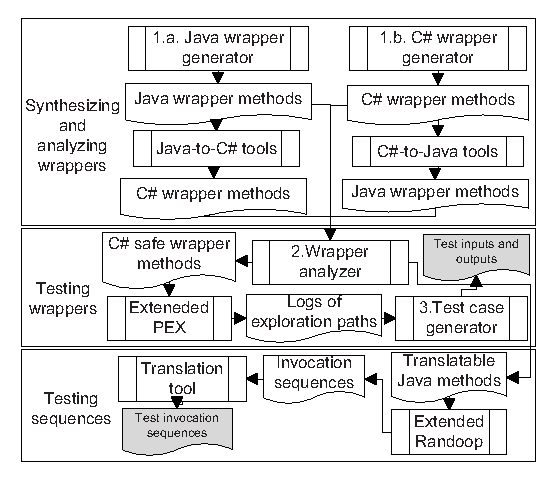
\includegraphics[scale=1,clip]{figure/approach.eps}\vspace*{-3ex}
 \caption{Overview of our approach}\vspace*{-3.5ex}
 \label{fig:approach}
\end{figure}

%-------------------------------------------------------------------
\subsection{Aligning Client Code}
\label{sec:approach:acc}

Initially, our approach accepts two versions of a project (one version in
$L_1$ and the other version in $L_2$) and aligns classes and methods
of the two versions. Aligned classes or methods
between the two versions implement a similar functionality. As they
implement a similar functionality, APIs used by these classes or methods can be
replaceable.

To align classes and methods of the two versions, our approach uses
name similarities between entities (such as class names or method names)
defined by the two versions of the project. In our approach, we have two
different kinds of entity names: entity names defined by the two versions
of the project and entity names of third-party libraries used by the two versions of the project.
The first kind often comes from the same programmer or the same team, or
programmers may refer to existing versions for naming entities such
as classes, methods, and variables. Therefore, name similarity is often
reliable to distinguish functionalities of the first kind compared to the second
kind. Our approach uses Simmetrics\footnote{\url{http://sourceforge.net/projects/simmetrics/}}
to calculate name similarities.

Algorithm 1 shows how our approach aligns client code classes. The
first step is to find candidate class pairs by names. For two sets
of classes ($C$ and $C'$), the algorithm returns candidate class
pairs ($M$) with a similarity greater than a given threshold,
referred to as \emph{SIM\_THRESHOLD}. As some projects may have many
classes with the same name, $M$ may contain more than one matching
pair for a class in a version. To align those classes, our algorithm
uses package names of these classes to refine $M$ and returns only
one matching pair with the maximum similarity\footnote{For C\#, we
refer to namespace names for package names.}.

In each aligned class pair, our approach further aligns methods
within the class pair. The algorithm for methods is similar to the
algorithm for classes but relies on other criteria such as the number of parameters
and names of parameters to refine candidate method pairs. These candidates
may contain more than one method pair due to overloading.
For the example shown in Section~\ref{sec:example}, our approach
correctly aligns the class \CodeIn{IndexFiles} and the method
\CodeIn{main} in Java to the class \CodeIn{IndexFiles}
and the method \CodeIn{Main} in C\# as their names are quite
similar.
%-----------------------------------------------------------------
\subsection{Mapping API classes}
\label{sec:approach:mappingtypes}

In this step, our approach mines mapping relations of
API classes. As defined in Section~\ref{sec:mapping}, mapping relations of API classes are used
to translate variables. Consequently, our approach mines mapping
relations of API classes based on how aligned client code declares
variables such as fields of aligned classes, parameters of aligned methods
and local variables of aligned methods. In
particular, for each aligned class pair $\Pair{c_1} {c_2}$, our
approach analyzes each field pair $\Pair{f_1}{f_2}$ and considers
$\Pair{f_1.type} {f_2.type}$ as one mined mapping relation of API
classes when the similarity between $f_1.name$ and $f_2.name$ is
greater than \emph{SIM\_THRESHOLD}. Similarly, for each aligned method pair
$\Pair{m_1} {m_2}$, our approach analyzes each local variable pair
$\Pair{var_1} {var_2}$ and considers $\langle var_1.type,$ $
var_2.type\rangle$ as one mined mapping relation of API classes when
the similarity between $var_1.name$ and $var_2.name$ is greater than
a threshold. Also, our approach analyzes each parameter pair
$\langle para_1, $ $para_2\rangle$ of $m_1$ and $m_2$, and our
approach considers $\langle para_1.type,$ $para_2.type\rangle$ as
one mined mapping relation of API classes when the similarity
between $para_1.name$ and $para_2.name$ is greater than \emph{SIM\_THRESHOLD}.

For the example shown in Section~\ref{sec:example}, our approach
mines the mapping relation between \CodeIn{java.io.File} and
\CodeIn{System.IO.FileInfo} based on the matched fields of Lines 4
and 9 (Figure~\ref{fig:clientcode}). The mapping relation of API classes helps translate the
variable declared in Line 1 (Figure~\ref{fig:totranslation})
to the variable declared in Line 16 (Figure~\ref{fig:translatedcode}).

%\begin{algorithm}[t]
%\begin{SmallOut}
%\dontprintsemicolon
%  \KwIn{$C$ is the classes of a language; $C'$ is the classes
%  of another language}
%  \KwOut{$P$ is aligned pairs of classes}
%  \Begin{
%     $M \leftarrow findCandidateClassPairs(C, C')$\;
%     \While{$M.size > 0 $}{
%        \If{$M.size > 1$}{
%            $M \leftarrow refineByPackageNames(M)$\;
%         }
%         \If{$M.size == 1$}{
%                $P.add(M)$\;
%                $C.remove(M[0].c)$\;
%                $C'.remove(M[0].c')$\;
%         }
%         $M \leftarrow findCandidateClassPairs(C, C')$\;
%     }
% }
%\end{SmallOut}
%\label{alg:alignclasses} \caption{Align Classes Algorithm}
%\end{algorithm}

\begin{figure}[t]
\centering
\includegraphics[scale=1,clip]{figure/algorithm1.eps}
\vspace*{-6ex}
\end{figure}

%-----------------------------------------------------------
\subsection{Mapping API methods}
\label{sec:approach:mappingtypes}

In this step, our approach mines mapping relations of API methods.
This step has two major sub-steps. First, our approach builds a graph, referred
as API transformation graph, for each client code
method. Second, our approach compares the two graphs of each paired
client code methods for mining mapping relations of API methods.

\begin{figure*}[t]
\centering
\includegraphics[scale=1.1,clip]{figure/graph.eps}\vspace*{-3ex}
 \caption
{\label{fig:graph}Built ATGs and the main steps of comparing
ATGs}\vspace*{-3.5ex}
\end{figure*}


\subsubsection{API transformation graph}
We propose API transformation graphs (ATG) to help deal with the two
challenges of mining API mapping listed in
Section~\ref{sec:introduction}. An API transformation graph of a
client code method $m$ is a directed graph
$G\Triple{N_{data}}{N_{m}}{E}$. $N_{data}$ is a set of the fields
$F$ of $m$'s declaring class, local variables $V$ of $m$, parameters
$P_1$ of $m$, parameters $P_2$ of methods called by $m$, and return
values $R$ of all methods. $N_{m}$ is a set of methods called by
$m$. $E$ is a set of directed edges. An edge $d_1\rightarrow d_2$
from a datum $d_1 \in N_{data}$ to a datum $d_2 \in N_{data}$
denotes the data dependency from $d_1$ to $d_2$. An edge $d_1
\rightarrow m_1$ from a datum $d_1 \in N_{data}$  to a method $ m_1
\in N_{m}$ denotes $d_1$ is a parameter or a related variable of
$m_1$. An edge $m_1 \rightarrow d_1$ from a method $m_1 \in N_{m}$
to a datum $d_1 \in N_{data}$ denotes $d_1$ is the return value of
$m_1$.

%We propose ATG for two main purposes. The first purpose is to mine mapping
%relations among parameters of mapped API methods. Mining mapping relations
%among parameters of mapped API methods is challenging as often mapped API methods
%can have different number of parameters or different positions among
%parameters. For example, consider the following two mapped API methods:
%
%\begin{CodeOut}
%$m_1$ in Java: BigDecimal java.math.BigDecimal.multiply (BigDecimal $p_1^1$)\\
%\hspace*{0.11in}$m_2$ in C\#: Decimal System.Decimal.Multiply (Decimal $p_1^2$, Decimal $p_2^2$)
%\end{CodeOut}
%
%Method $m_1$ of Java has a receiver variable, say $v_1^1$, of type \CodeIn{BigDecimal}
%and has one parameter $p_1^1$. The mapped method $m_2$ in C\# has
%two parameters $p_1^2$ and $p_2^2$. Using ATGs, our approach
%identifies that $v_1^1$ is mapped to $p_1^2$ and $p_1^1$ is mapped
%to $p_2^2$. As ATG captures parameters of API methods,
%our approach is able to deal with the challenges of mapping parameters.
%
%The second purpose of ATG is to mine mapping relations of merged API methods. As ATG
%describes data dependencies among inputs and outputs, our approach
%is able to mine mapping relations for merged API methods as shown in
%Figure~\ref{fig:example}. We next describe how our approach builds ATGs and
%uses ATGs for mining mapping relations of API methods.

\subsubsection{Building API transformation graphs }

Our approach builds an ATG for each method $m$. ATG includes information such as
inputs and outputs for each client code method. In particular, for
each method $m$, our approach first builds subgraph for its variables,
API methods, and field accesses according to the following rules:

%First, programming languages typically provide a huge set of APIs,
%and it is difficult to build mapping relations for all APIs
%manually. Second, some API methods have multiple parameters, and
%some parameters cannot be mapped directly one by one in orders. For
%example, \CodeIn{org.w3c.dom.Element.getAttributeNS()} and
%\CodeIn{System.Xml.XmlElement.GetAttribute()} both have two
%parameters, but the two parameters are inverse by their meanings.
%Third, one API method in one language may be mapped to more than one
%API method in other languages. For example, \CodeIn{java.util.
%LinkedList.removeLast()} returns the last value, and \CodeIn{System.
%Collections.Generic.LinkedList.RemoveLast()} does not return any
%values. To get that value, C\# programmers need to call more APIs,
%and thus one API method of Java is mapped to serval API methods of
%C\#.



%
%One challenge to mine mapping relations of two API methods lies in
%how to map their inputs correctly. Here, our approach both the
%receiver and the parameters of a method as the inputs of a
%method. Inputs of two API methods may be matched but are not in the
%same order. For example, as shown in Section~\ref{sec:example},
%\CodeIn{java.io. File.exist()} has a receiver whereas
%\CodeIn{System.IO.File.Exist()} has no receiver but a
%parameter. In addition, parameter orders may be quite different. For
%example, the parameter order of \CodeIn{org.w3c.
%dom.Element.getAttributeNS()} is inverse with the parameter order of
%\CodeIn{System.Xml.XmlElement.GetAttribute()}. To deal with the
%preceding problem,


\begin{enumerate}\vspace*{-2ex}
\item $\forall$ $f \in F \cup V \cup P_1$, our approach adds a node to the built ATG.
The reason for considering these variables such as fields in
declaring class or local variables in method $m$ used in client code
is that these variables are useful to analyze data dependencies
among API methods.\vspace*{-2ex}
%\begin{center}
%\includegraphics[scale=0.7,clip]{figure/rule1.eps}
%\end{center}
\item $\forall$ API methods of the form ``$T_0\ T.AM (T_1 p_1, \ldots, T_n p_n)$''
called by method $m$, our approach adds receiver (of type $T$) and
parameter nodes to the built ATG as shown below. Our approach does
not add receiver node for static API methods. \vspace*{-3ex}
\begin{center}
\includegraphics[scale=0.7,clip]{figure/rule2.eps}%\vspace*{-1.5ex}
\end{center}\vspace*{-3ex}
\item $\forall$ $f\in F \cup V$, if $f$ is a non-primitive variable
of type $T_1$ and a field $x$ of $T_1$ is accessed as $f.x$, our
approach adds nodes to the built ATG as shown below. As Java often
uses getters and setters whereas C\# often use field accesses, our
approach treats field accesses as a special type of method
calls.\vspace*{-2ex}
\begin{center}
\includegraphics[scale=0.7,clip]{figure/rule3.eps}%\vspace*{-1.5ex}
\end{center}\vspace*{-3ex}
\end{enumerate}

Our approach adds additional edges to the built ATG (and sub-graphs
inside ATG) representing data dependencies among built sub-graphs.
We use the following rules for adding additional edges to the built
ATG. \Comment{In particular, our approach analyzes source files of a
client code method statement by statement and adds edges according
to the rules as follows:} \vspace*{-1.5ex}
\begin{enumerate}
\item $\forall$ statements of the form $x = y$, where $x \in F \cup V \wedge y \in F \cup V$,
our approach adds an edge from $y$ to $x$. This edge represents that
$x$ is data dependent on $y$.\vspace*{-1.5ex}
\begin{center}
\includegraphics[scale=0.7,clip]{figure/rule4.eps}%\vspace*{-1.5ex}
\end{center}\vspace*{-1.5ex}
\item $\forall$ statements of the form $x = AM()$, where $x \in F \cup V$, our approach
adds an edge from $AM$ to $x$ if the return value of $AM$ is
assigned to $x$. This edge represents that $x$ is data dependent on
the return value of $AM$. \vspace*{-1.5ex}
\begin{center}
\includegraphics[scale=0.7,clip]{figure/rule5.eps}%\vspace*{-1.5ex}
\end{center}\vspace*{-1.5ex}
\item $\forall$ API methods $AM(x)$ called by method $m$, our approach
adds an edge from $x$ to the parameter node of $AM$. This edge
represents that the parameter of $AM$ is data dependent on
$x$.\vspace*{-1.5ex}
\begin{center}
\includegraphics[scale=0.7,clip]{figure/rule6.eps}%\vspace*{-1.5ex}
\end{center}\vspace*{-1.5ex}
\item $\forall$ statements of the form $m_2(m_1(x))$, our approach
adds an edge from the return value node of $m_1$ to the parameter
node of $m_2$ parameter node. This edge represents that the
parameter of $m_2$ is data dependent on the return value of
$m_1$.\vspace*{-1.5ex}
\begin{center}
\includegraphics[scale=0.7,clip]{figure/rule7.eps}%\vspace*{-1.5ex}
\end{center}\vspace*{-1.5ex}
\item $\forall$ statements of the form $x.m()$, our approach adds
an edge from $x$ to $m$ as $x$ is the receiver object of $m$. This
edge represents that the receiver object of $m$ is data dependent on
$x$.\vspace*{-1.5ex}
\begin{center}
\includegraphics[scale=0.7,clip]{figure/rule8.eps}%\vspace*{-1.5ex}
\end{center}\vspace*{-1.5ex}
\item $\forall$ statements of the form $ x = y\ op\ z\ op\ \ldots, op \in \{+,-,*,/\}$,
our approach adds edges from $y$, $z$, and others to $x$, as these
variables are connected by binary operations and the return value is
assigned to $x$. The edge denotes the data dependency from $y$, $z$,
and other variables to $x$. For simplicity, our approach ignores
\emph{op} info. We discuss the issue in
Section~\ref{sec:discuss}.\vspace*{-1.5ex}
\begin{center}
\includegraphics[scale=0.7,clip]{figure/rule9.eps}%\vspace*{-1.5ex}
\end{center}\vspace*{-2ex}
\end{enumerate}

For each method $m$ in the client code, our approach applies preceding
rules for each statement from the beginning to the end of $m$.
Within each statement, our approach applies these rules based on
their nesting depth in the abstract syntax tree. For example,
for the statements of the form $m_2(m_1(x))$, our approach first applies
these rules on $m_1$ and then on $m_2$.

Figures~\ref{fig:graph}a and ~\ref{fig:graph}b show partial ATGs for
C\# (\CodeIn{IndexFiles.cs}) and Java (\CodeIn{IndexFiles.java})
code examples shown in Figure~\ref{fig:clientcode}, respectively.
Figure~\ref{fig:graph} also shows corresponding line numbers of each
sub-graph. Our approach applies Rules 2 and 6 for Lines 4 and 9 (Figure~\ref{fig:clientcode})
to build corresponding sub-graphs in the ATG. For
Lines 6 and 7 (Figure~\ref{fig:clientcode}), our approach applies Rules 2 and 8 to build
corresponding sub-graphs in the ATG. For Lines 12 and 15 (Figure~\ref{fig:clientcode}),
our approach applies Rule 2, 3, and 6 to build corresponding sub-graphs.

%\begin{algorithm}[t]
%\begin{SmallOut}
%\label{alg:mapATG} \dontprintsemicolon
%  \KwIn{$G$ is the ATG of a method ($m$); $G'$ is the ATG of $m$'s mapped method.}
%  \KwOut{$S$ is a set of mapping relations for API methods}
%  \Begin{
%     $P \leftarrow findVarPairs(m, m')$\;
%     \For{Pair p in P}{
%        $SM \leftarrow G.nextMethods(p.sharp)$\;
%        $JM \leftarrow G.nextMethods(p.java)$\;
%        $\Delta S = mapping(SM, JM)$\;
%        \While{$\Delta S \neq \phi| \Delta SM \neq \phi| \Delta JM \neq \phi$}{
%            $S.addAll(\Delta S)$\;
%             \For{Method sm in SM}{
%                 \If{$sm.isMapped$}{
%                    $SM.replace(sm, sm.nextMethod())$\;
%                  }\Else{
%                    $SM.replace(sm, sm.mergeNextMethod())$\;
%                  }
%             }
%             \For{Method jm in JM}{
%                 \If{$jm.isMapped$}{
%                    $JM.replace(jm, jm.nextMethod())$\;
%                  }\Else{
%                    $JM.replace(jm, Jm.mergeNextMethod())$\;
%                  }
%             }
%             $\Delta S = mapping(SM, JM)$\;
%        }
%     }
% }
% \end{SmallOut}
%\caption{ATG Comparison Algorithm}
%\end{algorithm}

\begin{figure}[t]
\centering
\includegraphics[scale=1,clip]{figure/algorithm2.eps}
\vspace*{-6ex}
\end{figure}

%--------------------------------------------------------------------
\subsubsection{Comparing API transformation graphs}

The second sub-step compares each pair of built ATGs for mining mapping
relations of API methods. Our mapped API methods satisfy three
criteria: (1) Mapped API methods implement the same
functionality. (2) Mapping relation describes the relation
between parameters of mapped API methods. (3) Mapping relation
describes the relation between return values of
mapped API methods. The two mapped API methods in two
different languages satisfying the preceding three criteria
are replaceable in the client code. Therefore, these mapped API
methods assist for migrating client code from one language to another.

Algorithm 2 presents major steps of comparing ATGs for mining
mapping relations of API methods. Consider two methods $m$ and $m'$
of two different languages $L$ and $L'$, respectively, in the client
code. Consider that the associated ATGs of $m$ and $m'$ are compared
to mine mapping relations of API methods. First, our algorithm finds
matching variables $\in$ $F$, $V$, and $P_1$ in $m$ and $m'$. Our
algorithm maps two variables $v$ and $v'$ of methods $m$ and $m'$,
respectively, if the similarity measure on their names is greater
than \emph{SIM\_THRESHOLD}. For constants in $m$ and $m'$, our
algorithm maps those two constants, if they have exactly the same
value. Our algorithm uses these variable and constant mappings to
compute mappings between API methods that use these variables and
constants. Our algorithm uses the following criteria for mapping two
API methods $jm$ and $sm$.

\emph{Matching entities}: The first criterion is based on entities such as receiver variable
or parameters of $jm$ and $sm$ to map $jm$ and $sm$. We map $jm$ with $sm$, if
the receiver variable of API method $jm$ is mapped
to the receiver variable of $sm$, and there is a one-to-one mapping between parameters
of $jm$ and $sm$.

\emph{Matching functionalities}: The second criterion is based on functionalities of
$jm$ and $sm$. We consider that $jm$ and $sm$ implement the same functionality,
if the similarity measure between the name of $jm$ and the name of $sm$ is
greater than \emph{SIM\_THRESHOLD}.

\emph{Matching outputs:} The third criterion is based on the return values of $jm$ and $sm$.
Consider the return values of $jm$ and $sm$ as $r_1$ and $r_2$, respectively. We map $jm$
with $sm$, if the type of $r_1$ is mapped with the type of $r_2$ in mapping API classes
relationship.

Our algorithm first attempts to map first API method $jm$ in $m$
with the first API method $sm$ in $m'$. If our algorithm successfully maps $jm$ with
$sm$, our algorithm moves to the next available API methods in $m$
and $m'$ of the client code. If our algorithm does not able to map $jm$
with $sm$, our algorithm merges $sm$ and $jm$ with their next available API methods
in the corresponding ATGs, respectively, and attempts to map merged API methods.
For two merged API methods, our algorithm uses the
maximum similarity of method names between $jm$ and $sm$ as a
similarity measure for matching their functionalities.
With each iteration, $sm$ or $jm$ or the mapping relation (represented as $S$)
in the algorithm changes. Therefore, we repeat our algorithm
till $S$, $sm$, and $jm$ do not change anymore.

We next explain our algorithm using the illustrative example shown
in Figure~\ref{fig:graph}. The numbers shown in circles
represent the major steps in our algorithm for mining mapping
relations of API methods. We next explain each step in detail.

\emph{S1: mapping parameters, fields, local variables, and constants.}
Given two ATGs of each method pair $\langle m, m' \rangle$, this step maps
variables such as parameters, fields, and local variables by comparing their names
and maps constants by comparing their values. As shown in
Figure~\ref{fig:graph}, Step 1 maps two constants as both the constants
have the same value \CodeIn{index}.

\emph{S2: mapping inputs of API methods.} Step 2 mines mapping
relations of API methods using variable and constant mapping relations.
Initially, this step identifies first API methods in the two ATGs and tries to
map their parameters and receiver objects of the two API methods.
In our current example, this step maps the parameter \CodeIn{filename}
to the parameter \CodeIn{arg0} as these parameters
are of the same type and their associated constants are mapped.

\emph{S3: mapping outputs of API methods.} In contrast to Step 2
that maps parameters, Step 3 maps return values of API methods. In
this step, if our approach is not able to map return values, our
approach merges the next API method and then attempts to map return
values of merged API methods. In our current example shown in
Figure~\ref{fig:graph}, return value of
\CodeIn{System.IO.FileInfo.FileInfo()} cannot be mapped to the
return value of \CodeIn{java.io.File.File()}. Therefore, our
approach merges next API methods in the ATG till the \CodeIn{Exists}
API method, as the return values (shown as \CodeIn{Boolean}) match
only after the \CodeIn{Exists} API method. Figure~\ref{fig:graph}
shows Step 3 along with the matching return values.

\emph{S4: mapping functionalities.} After our approach maps parameters and return values,
this step further maps functionalities of those merged API
methods. Given two merged API methods with mapped parameters and return values,
this step uses the similarity measure based of their method names as a criterion
for matching their functionalities. In the preceding example, this step maps
the two merged API methods shown in Figure~\ref{fig:graph}a to the
merged API methods of the \CodeIn{java.io.File.exist()} as all three
merged API methods include the method named \CodeIn{exist}.

Our approach applies preceding steps on ATGs
(as shown in Figures~\ref{fig:graph}a and~\ref{fig:graph}b) and mines
mapping relations. An example mapping relation from the preceding ATGs is
shown in Figure~\ref{fig:example}.
\vspace*{-1ex}
\begin{table}[t]
\centering
\begin{SmallOut}
\begin {tabular} {|c|r|r|r|r|r|r|r|}
 \hline
\multirow{2}*[-2pt]{\textbf{Type}}&
\multicolumn{1}{|c}{\multirow{2}*[-2pt]{\textbf{Num}}}
& \multicolumn{2}{|c|}{\textbf{Java2CSharp}} & \multicolumn{2}{|c|}{\textbf{JLCA}}& \multicolumn{2}{|c|}{\textbf{sharpen}} \\\cline{3-8} &  &  \textbf{M}& \textbf{\%} &  \textbf{M}& \textbf{\%}&  \textbf{M}& {\%}\\
\hline
sfg  &  16962 & 237 & 1.4\% & 3744 & 22.1\% & 47 & 0.3\%\\
\hline
sfs  &  0    & 0    & n/a   & 0    & n/a    & 0  & n/a  \\
\hline
nfg  &  832  & 0    & 0.0\% & 121  & 14.5\% & 0  & 0.0\%\\
\hline
nfs  &  823  & 0    & 0.0\% & 79   & 9.6\%  & 0   & 0.0\%\\
\hline
sm   &1175   & 97   & 8.3\% & 198  & 16.9\% & 26  & 2.2\%\\
\hline
nm   &175400 & 3589 & 2.0\% & 39536& 22.5\% & 1112& 0.6\%  \\
\hline
Total &195192& 3923 &  2.0\% & 43678 & 22.4\% & 1185 & 0.6\%\\
\hline
\end{tabular}\vspace*{-2ex}
\Caption{Translation results of Java-to-C\# tools} \label{table:java2csharp}
\end{SmallOut}\vspace*{-4ex}
\end{table}
\section{Evaluations}
\label{sec:evaluation}

We implemented a tool for TeMAPI and conducted evaluations using our tool to address the following research questions:

\vspace*{-1.5ex}
\begin{enumerate}
%\item How effectively can existing translation tool translate API elements (Section~\ref{sec:evaluation:element})? \vspace*{-1.8ex}
\item How many API elements can be translated by existing translation tools (Section~\ref{sec:evaluation:element})? \vspace*{-1.8ex}
%\item How effectively can our approach detect behavioral differences of single API classes (Section~\ref{sec:evaluation:single})?\vspace*{-1.8ex}
\item How many behavioral differences of single API classes are effectively detected by our approach (Section~\ref{sec:evaluation:single})?\vspace*{-1.8ex}
%\item How effectively can our approach detect behavioral differences of multiple API classes (Section~\ref{sec:evaluation:single})?\vspace*{-1.8ex}
\item How many behavioral differences of multiple API classes are effectively detected by our approach (Section~\ref{sec:evaluation:sequence})?\vspace*{-1.8ex}
%\item Can the our combination strategy helps achieve better coverage (Section~\ref{sec:evaluation:coverage})?
\item How many behavioral differences are detected with TeMAPI's internal techniques on and off (Section~\ref{sec:evaluation:techniques})?
\end{enumerate}\vspace*{-1.5ex}

Table~\ref{table:subjects} shows used subject tools. Column ``Name'' lists names of subject tools. We use \emph{converter} to denote the ``VB \& C\# to Java converter'' for short. Column ``Version'' lists versions of subject tools. Column ``Provider'' lists companies of subject tools. Although all these tools are from commercial companies, Java2CSharp, sharpen, and Net2Java are open source tools. Column ``Description'' lists main functionalities of subject tools. We choose these tools as subjects, since they are popular and many programmers recommend these tools in various forums.

All evaluations were conducted on a PC with Intel Qual CPU @ 2.83GHz and 2G memory running Windows XP.

\subsection{Translating Synthesized Wrappers}
\label{sec:evaluation:element}
This evaluation focuses on the effectiveness of our approach to extract API mapping relations from both open source tools and closed source tools. The results are useful to follow-up steps, and also reveal to what extents existing translation tools can support API translation. For Java-to-C\# tools, TeMAPI first synthesized wrapper methods for all classes of J2SE 6.0\footnote{\url{http://java.sun.com/javase/6/docs/api/}}. During synthesizing,  TeMAPI ignored all generic API methods as described in Section~\ref{sec:approach:single}, and Table~\ref{table:java2csharp} shows the translation results. Column ``Type'' lists types of synthesized methods: ``sfg'' denotes getters of static fields; ``sfs'' denotes setters of static fields; ``nfg'' denotes getters of non-static fields; ``nfs'' denotes setters of non-static fields; ``sm'' denotes static methods; ``nm'' denotes non-static methods; and ``Total'' denotes the sum of all methods. Column ``Num'' lists numbers of corresponding types of methods. Columns ``Java2CSharp'', ``JLCA'', and ``sharpen'' list the translation results of corresponding translation tools, respectively. For these columns, sub-columns ``M'' and ``\%'' list the number and percentage of translated wrapper methods without compilation errors, respectively.


Our results show that it is quite challenging for a translation tool to cover all API elements, since API elements are quite large in size. Although JLCA can translate 43,678 wrapper methods, these methods cover only 22.4\% of total number of wrapper methods. Furthermore, even if an API element is translated, it can be translated to an API element with a different behavior. We observe that developers of translation tools may already aware of these behavioral differences. For example, after JLCA translated synthesized code, it generated a report with many warning messages regarding behavioral differences of translated API elements. For example, a warning message is ``Method \CodeIn{java.lang.String.indexOf} was converted to \CodeIn{System.String.IndexOf}, which may throw an exception'', but the report does not tell programmers when such an exception is thrown or how to deal with that exception. TeMAPI complements the problem, and detects that the Java method does not check whether inputs are out of ranges as the C\# method does. For example, given an empty string \CodeIn{str}, the \CodeIn{str.lastIndexOf("", 1)} statement in Java returns 0, whereas the \CodeIn{str.LastIndexOf("", 1)} statement in C\# throws \CodeIn{ArgumentOutOfRangeExcpetion}.

\begin{table}[t]
\centering
\begin{SmallOut}
\begin {tabular} {|c|r|r|r|r|r|c|c|}
 \hline
\multirow{2}*[-2pt]{\textbf{Type}}&
\multicolumn{1}{|c}{\multirow{2}*[-2pt]{\textbf{Num}}}
& \multicolumn{2}{|c|}{\textbf{Net2Java}} & \multicolumn{2}{|c|}{\textbf{converter}}\\\cline{3-6} &  &  \textbf{M}& \textbf{\%} &  \textbf{M}& \textbf{\%}\\
\hline
sfg  &  3223 & 1    & 0.0\% & 3    & 0.1\% \\
\hline
sfs  &  8    & 0    & 0.0\% & 0    & 0.0\%   \\
\hline
nfg  &  117  & 0    & 0.0\% & 0    & 0.0\%\\
\hline
nfs  &  115  & 0    & 0.0\% & 0    & 0.0\%\\
\hline
sm   &996    & 4   & 0.4\% & 6  & 0.6\% \\
\hline
nm   &190376 & 94    & 0.0\% & 387    & 0.2\% \\
\hline
Total &194835& 99   &  0.1\% & 396 & 0.2\%\\
\hline
\end{tabular}\vspace*{-2ex}
\Caption{Translation results of C\#-to-Java tools} \label{table:csharp2java}
\end{SmallOut}\vspace*{-4ex}
\end{table}

For C\#-to-Java translation tools, TeMAPI first synthesized wrapper methods for all classes of the .NET framework client profile\footnote{\url{http://tinyurl.com/252t2ax}}. As described in Section~\ref{sec:approach:single}, besides generic methods, TeMAPI also ignored \CodeIn{unsafe} methods, \CodeIn{delegate} methods, and methods whose parameters are marked with \CodeIn{out} or \CodeIn{ref}. TeMAPI synthesized almost the same size of wrapper methods as synthesized for J2SE 6.0. Table~\ref{table:csharp2java} shows the translation results. We find that both tools translate only a small number of API elements. One primary reason could be that C\# provides many features such as partial class, reference parameters, output parameters, and named arguments, that are not provided by Java\footnote{\url{http://tinyurl.com/yj4v2m2}}. We suspect that a C\#-to-Java translation tool needs take these issues into consideration, so many mapping relations of API elements are not addressed yet.

Tables~\ref{table:java2csharp} and~\ref{table:csharp2java} show that Java-to-C\# tools cover much more API elements compared to C\#-to-Java tools. To give more insights, we next present more details at the package level regarding the translation results of Java-to-C\# tools in Table~\ref{table:package}. Column ``Name'' lists names of Java packages. To save space, we omit the prefixes such as ``java.'', ``javax.'', and ``org.''. We also use short names ``acc.'', ``man.'', ``java.sec.'', and ``javax.sec.'' to represent \CodeIn{javax.accessibility}, \CodeIn{javax.management}, \CodeIn{java.security}, and \CodeIn{javax.security} packages, respectively. Besides, we omit 12 packages that are not covered by all the three tools (\emph{e.g.}, the \CodeIn{javax.rmi} package). Table~\ref{table:package} shows that all the three translation tools cover four packages: \CodeIn{java.io}, \CodeIn{java.lang}, \CodeIn{java.util}, and \CodeIn{java.net}. The four packages seem to be quite important for most Java programs. Almost for all these packages, JLCA covers more API elements than the other two tools. JLCA even covers GUI-related packages such as the \CodeIn{java.awt} package and the \CodeIn{javax.swing} package. As a result, JLCA can translate some Java programs with GUI interfaces whereas the other two tools cannot.
\begin{table}[t]
\centering
\begin{SmallOut}
\begin {tabular} {|p{3.6em}|r|r|r|r|r|r|r|}
 \hline
\multicolumn{1}{|c}{\multirow{2}*[-2pt]{\textbf{Name}}}&
\multicolumn{1}{|c|}{\multirow{2}*[-2pt]{\textbf{Num}}}
& \multicolumn{2}{|c|}{\textbf{Java2CSharp}} & \multicolumn{2}{|c|}{\textbf{JLCA}}& \multicolumn{2}{|c|}{\textbf{sharpen}} \\\cline{3-8} &  &  \textbf{M}& \textbf{\%} &  \textbf{M}& \textbf{\%}&  \textbf{M}& {\%}\\
\hline
awt  &  29199  & 0     &  0.0\%  &  8637  &  29.6\%  &  0   & 0.0\%\\
\hline
bean &  \hfill 1768   & 20    &  1.1\%  &  14    &  0.8\%   &  0   & 0.0\% \\
\hline
io   &  \hfill 3109   & 592   &  19.0\% & 1642   &  52.8\%  & 43   & 1.4\%\\
\hline
lang &  \hfill 5221   & 1494  &  28.6\% & 2377   &  45.5\%  & 791  & 15.2\%\\
\hline
math &  \hfill 1584   & 101   &  6.4\%  & 232    &  14.6\%  & 0    & 0.0\%\\
\hline
java.net  &  \hfill 1990   & 52    &  2.6\%  & 482    &  24.2\%  & 10   & 0.5\%  \\
\hline
nio  &  \hfill 536    & 30    &  5.6\%  & 0      &  0.0\%  &  0    & 0.0\%  \\
\hline
java.rmi  &  \hfill 1252   & 0     &  0.0\%  &  707   &  56.5\%  &  0   & 0.0\%\\
\hline
java.sec. &  \hfill 2797   & 50    &  1.8\%  &  702    &  25.1\%   &  0   & 0.0\% \\
\hline
java.sql   &  \hfill 3495   & 20   &  0.6\% & 183   &  5.2\%  & 0   & 0.0\%\\
\hline
text  &  \hfill 1068   & 96   &  9.0\% & 321   &  30.1\%  & 0  & 0.0\%\\
\hline
util  &  \hfill 9586   & 1372   &  14.3\%  & 1879    &  19.6\%  & 341    & 3.6\%\\
\hline
acc.  &  \hfill 237   & 1    &  0.4\%  & 25    &  10.5\%  & 0   & 0.0\%  \\
\hline
activation     &  \hfill 538   & 0    &  0.0\%  & 165   &  30.7\%  & 0   & 0.0\%  \\
\hline
crypto        &  \hfill 625   &  0    &  0.0\%  &  263  &  42.1\%  &  0    & 0.0\%\\
\hline
man.   &  \hfill 5380   & 2    &   0.0\%  & 0     &  0.0\%  & 0    & 0.0\%  \\
\hline
naming       &  \hfill 3565   & 0    &   0.0\%  & 1365   &  38.3\%  &  0    & 0.0\%  \\
\hline
javax.sec.       &  \hfill 1435  & 0     &  0.0\%  & 619     &  43.1\%  & 0    & 0.0\%\\
\hline
sound          &  \hfill 515   & 0    &  0.0\%  & 56    &  10.9\%  & 0   & 0.0\%  \\
\hline
swing          &  102389& 10   &  0.0\%  &  21364 &  20.9\%   &  0   & 0.0\%\\
\hline
javax.xml            &  \hfill 4188  &  34   &  0.8\% &  580   &  13.8\%  & 0  & 0.0\%\\
\hline
org.omg              &  \hfill 8937   & 0    &  0.0\%  & 1578  &  17.7\%  & 0   & 0.0\%  \\
\hline
w3c.dom          &  \hfill 83     & 0    &  0.0\%  & 14     &  16.9\%   & 0   & 0.0\%  \\
\hline
org.xml             &   \hfill 897    & 49   &  5.5\%  & 473    & 52.7\%    & 0   & 0.0\%\\
\hline
\end{tabular}\vspace*{-2ex}
\Caption{Java-to-C\# translation results at package level} \label{table:package}
\end{SmallOut}\vspace*{-5ex}
\end{table}
%------------------------------------------------------------
\subsection{Testing Single Classes}
\label{sec:evaluation:single}

To detect behavioral differences of single classes, TeMAPI leverages Pex to explore safe wrapper methods. These methods include both the translated C\# wrapper methods without compilation errors (as shown in Table~\ref{table:java2csharp}) and the synthesized C\# wrapper methods that can be translated into Java without compilation errors (as shown in Table~\ref{table:csharp2java}). During exploration, when Pex generates inputs that exercise a feasible path in the wrapper method, TeMAPI records the inputs and resulting outputs of that path. Based on these inputs and outputs, TeMAPI generates Java test cases to ensure that synthesized wrapper methods and translated wrapper methods return the same outputs given the same inputs. Since testing GUI related API elements requires human interactions, we filter out GUI related API elements (\emph{i.e.}, the \CodeIn{awt} package and the \CodeIn{swing} package). In addition, when Pex explores methods without return values, we ignore paths that do not throw any exceptions, since we cannot generate Java related test cases. We discuss this issue in Section~\ref{sec:discuss}.

Table~\ref{table:singleinvoc} shows the results of executing generated Java test cases. Column ``Name'' lists names of translation tools. Column ``Num'' lists the number of generated Java test cases. Columns ``E-Tests'' and ``A-Tests'' list the number of exception-causing and assertion-failing test cases. These test cases reflect behavioral differences between mapped API elements. Among these two columns, sub-columns ``M'' and ``\%'' list the number and percentages of these test cases. Table~\ref{table:singleinvoc} shows that only about half of the generated Java test cases are passed. Among the five tools, sharpen includes the lowest number of ``E-Tests'' and ``A-Tests''. It seems that programmers of sharpen put great efforts to fix behavioral differences. The percentage of JLCA is also relatively low. The results are comparable, since JLCA translates much more API elements than the other tools. In total, about 50\% of test cases are failed. These results show the effectiveness of TeMAPI, since these test cases represent behavioral differences.



For Java2CSharp, JLCA, and sharpen, we further present their testing results at the package level in Table~\ref{table:packagetest}. Column ``Name'' lists names of J2SE packages. For columns ``Java2CSharp'', ``JLCA'', and ``sharpen'', sub-column ``R'' lists numbers of generated Java test cases, and sub-column ``\%'' lists percentages of failing test cases (including exception-causing and assertion-failing). Table~\ref{table:packagetest} shows that for the \CodeIn{java.sql} and \CodeIn{java.util} packages, all tools suffer from relatively high percentages of failing test cases, and for the \CodeIn{java.lang} and \CodeIn{java.math} packages, all tools include relatively low percentage of failing test cases. These results may reflect that some packages between Java and C\# are more similar than the others, so they can be more easily mapped. We also find that for the \CodeIn{java.text}, \CodeIn{javax.xml}, and \CodeIn{org.xml} packages, JLCA includes the lowest percentage of failing test cases among the five tools. The results indicate that a translation tool can achieve better translation results if the programmers carefully prepare mapping relations of API elements.

Tables~\ref{table:singleinvoc} and~\ref{table:packagetest} show that a high percentage of generated Java test cases are failed. To better understand behavioral differences of mapped API elements, we inspected 3759 failing Java test cases. For Net2Java and converter, we inspect all failing test cases, whereas for Java2CSharp, JLCA, and sharpen, we inspect test cases generated for the \CodeIn{java.lang} package, due to a large number of failing test cases. We next present our findings ranked based on the number of failing test cases.

\textbf{Finding 1:} 36.8\% test cases show the behavioral differences caused by \CodeIn{null} inputs.

We find that Java API methods and their translated C\# API methods can have behavioral differences when \CodeIn{null} values are passed as inputs. In some cases, a Java API method can accept \CodeIn{null} values, but its translated C\# API method throws exceptions. One such example is shown in Section~\ref{sec:example} (\emph{i.e.}, the \CodeIn{skip(long)} method). In other cases, a Java API method throws exceptions given a \CodeIn{null} input, but its translated C\# API method can accept \CodeIn{null} values. For example, JLCA translates the \CodeIn{java.lang.Integer.parseInt (String,int)} method in Java to the \CodeIn{System.Convert.ToInt32 (string,int)} in C\#. If the inputs of the Java method are \CodeIn{null} and $10$, it throws \CodeIn{NumberFormatException}, but given the same inputs, the output of the C\# method is 0. We notice that some translation tools can fix some differences caused by \CodeIn{null} inputs. For example, to fix the behavioral difference of \CodeIn{null} inputs for the \CodeIn{valueOf(Object)} method as shown in Section~\ref{sec:approach:single}, sharpen translates the method to its self-developed C\# method, and thus fix the difference.

\Comment{We also find that given the same inputs, a method may produce null outputs, whereas its mapped method will not. For example, converter maps the \CodeIn{Sys- tem.Collections.Queue.ToArray()} in C\# to the \CodeIn{java.util. LinkedList.toArray()} method in Java. Given an empty list, the C\# method produce a null value, whereas the Java method produce an empty array.}

\textbf{Implication 1:} Although implementers of API libraries in different languages can come to agreements on functionalities of many API methods, behaviors for \CodeIn{null} inputs are typically controversial. Some translation tools such as sharpen try to fix these differences, however, many such differences are still left to programmers as shown in our results. Therefore, programmers should be careful when inputs are \CodeIn{null}.

\begin{table}[t]
\centering
\begin{SmallOut}
\begin {tabular} {|c|r|r|r|r|r|c|c|}
 \hline
\multirow{2}*[-2pt]{\textbf{Name}}
& \multirow{2}*[-2pt]{\textbf{Num}} & \multicolumn{2}{|c|}{\textbf{E-Tests}}& \multicolumn{2}{|c|}{\textbf{A-Tests}} \\\cline{3-6}  &  & \textbf{M}& \textbf{\%} &  \textbf{M}& \textbf{\%}\\
\hline
Java2CSharp  &   15458 & 5248 & 34.0\% & 3261 & 21.1\% \\
\hline
JLCA         &   33034 & 8901 & 26.9\% & 6944 & 21.0\% \\
\hline
sharpen      &  2730 & 662  & 24.2\% & 451  & 16.5\%\\
\hline
net2java     &   352 & 40   & 11.4\%  & 261   & 74.1\%\\
\hline
converter    &  762 & 302  & 39.6\% & 182   & 23.9\%\\
\hline
Total        &  52336  &  15153 & 29.0\% &11099 & 21.2\%  \\
\hline
\end{tabular}\vspace*{-2ex}
\Caption{Results of testing single classes} \label{table:singleinvoc}
\end{SmallOut}\vspace*{-6ex}
\end{table}
\begin{table}[t]
\centering
\begin{SmallOut}
\begin {tabular} {|p{3.4em}|r|r|r|r|r|r|r|r|r|r|}
 \hline
\multicolumn{1}{|c}{\multirow{2}*[-2pt]{\textbf{Name}}}
& \multicolumn{2}{|c|}{\textbf{Java2CSharp}} & \multicolumn{2}{|c|}{\textbf{JLCA}}& \multicolumn{2}{|c|}{\textbf{sharpen}} \\\cline{2-7} &  \textbf{R}&  \textbf{\%} &   \textbf{R}& \textbf{\%} & \textbf{R}&   \textbf{\%}\\
\hline
bean &  \hfill 17     &    82.4\%  &  18        &  33.3\%   &  0      & n/a \\
\hline
io   &  \hfill 4155   &  67.8\%  &  6981       &  58.0\%   &   33    & 39.4\%\\
\hline
lang &  \hfill 3480   &   37.5\%  &  4431      &  26.1\%   &   1753 & 29.3\%\\
\hline
math &  \hfill 561    &   4.3\%  &   1629     &   1.5\%   &  0      & n/a\\
\hline
java.net  &   438     &   25.1\% &   3941     &   47.8\%  & 9       & 44.4\%  \\
\hline
nio  &  \hfill 27     &  48.1\% &    0        &   n/a     &  0     &  n/a \\
\hline
java.rmi  &  \hfill 0   &   n/a   &   884     &   32.6\%  &  0     & n/a\\
\hline
java.sec. &  \hfill 45  &   55.6\%  &  828    &  35.6\%   &  0    & n/a \\
\hline
java.sql   &  \hfill 260&   88.1\%  & 1465    &  91.0\%   &   0     & n/a\\
\hline
text  &  \hfill 566   &   61.5\%  & 374      &  18.2\%   & 0      & n/a\\
\hline
util  &  \hfill 5519  &   60.8\%  & 6177     & 70.2\%  & 935      & 62.4\%\\
\hline
acc.  &  \hfill 1    &   0.0\%   & 25         & 16.0\%    & 0          & n/a \\
\hline
activation  &  0     &    n/a    & 694      & 53.9\% & 0           & n/a  \\
\hline
crypto      &  0     &     n/a    & 298     & 24.2\% &  0        & n/a\\
\hline
man.        &  2     &    0.0\%  & 0        & n/a    &  0          & n/a  \\
\hline
naming      &  0     &    n/a     & 1569    & 40.6\%  &  0         & n/a  \\
\hline
javax.sec.  &  0     &   n/a     & 683     & 29.4\%  &  0        & n/a\\
\hline
sound       &  0     &   n/a     & 66       & 36.4\%  &   0        &n/a  \\
\hline
javax.xml   &  110   &    71.8\%  &  628    & 45.9\%  &   0         & n/a\\
\hline
org.omg     &  0     &   n/a     & 1842    & 36.3\%  & 0           & n/a  \\
\hline
w3c.dom     &  0     &   n/a     & 18      & 33.3\%  &  0         & n/a  \\
\hline
org.xml     &   277  &   70.0\%  & 483     & 27.3\%  & 0         & n/a\\
\hline
\end{tabular}\vspace*{-2ex}
\Caption{Java-to-C\# testing results of package level } \label{table:packagetest}
\end{SmallOut}\vspace*{-4ex}
\end{table}

\textbf{Finding 2:} 22.3\% test cases show the behavioral differences caused by stored string values.

We find that string values stored in fields between Java classes and their translated C\# classes are typically different. This difference ranks as the second, since each Java class has a \CodeIn{toString()} method and each C\# class also has a \CodeIn{ToString()} method. Many translation tools map the two API methods, but the return values of the two methods are quite different in many cases. Besides, many API classes declare methods like \CodeIn{getName} or \CodeIn{getMessage}. These methods also return string values that can be quite different. In particular, we find that the \CodeIn{Message} fields of exceptions in C\# often return informative messages. One such message is ``Index was outside the bounds of the array'' provided by the \CodeIn{System.Index- OutOfRangeException.Message} field in C\#. On the other hand, exceptions in Java often provide only \CodeIn{null} messages. Overall, we find that none of the five tools fixes this difference.

\textbf{Implication 2:} String fields of mapped classes in different languages typically store different values, but existing translation tools do not fix those differences. Programmers should not rely on these values, since they are typically different across languages.

\textbf{Finding 3:} 11.5\% test cases show the behavioral differences caused by illegal inputs or inputs out of ranges.

We find that API methods in Java seldom check whether their inputs are illegal or out of range, whereas API methods in C\# often do. For example, the \CodeIn{java.lang.Boolean.parseBoolean (String)} method in Java does not check for illegal inputs, and returns \CodeIn{false} given an illegal input such as ``\CodeIn{test}''. Java2CSharp translates it into the \CodeIn{System.Boolean.Parse(String)} method in C\#. The C\# method throws \CodeIn{FormatException} given the same input since it checks for illegal inputs. As another example, the \CodeIn{java.lang.Double.shortValue()} method in Java accepts values that are larger than 32,767. JLCA translates the Java method to the \CodeIn{Convert.ToInt16(double)} method in C\#. The C\# method throws \CodeIn{OverflowException} when values are larger than 32,767 since it checks whether inputs are too large.

\textbf{Implication 3:} API methods across languages may follow different standards to check their inputs for different considerations. If a tool translates code from a low standard to a high standard (\emph{e.g.}, Java to C\#), it can add extra code to satisfy the high standard. When programmers migrate from one language to another, they should check whether the new language follow a high standard or not.

\textbf{Finding 4:} 10.7\% test cases show the behavioral differences caused by different understanding.


We find that implementers of API libraries may have different understanding for mapped API methods in different languages. Two such examples are shown in Section~\ref{sec:approach:single} (\emph{i.e.}, the \CodeIn{capacity()} method and the \CodeIn{length()} method). In some cases, such differences reflect different natures between languages. For example, we find that Java considers ``\CodeIn{\textbackslash}'' as existing directories, but  C\# considers it not. In some other cases, we find that such differences can indicate defects in translation tools. For example, Java2CSharp translates the \CodeIn{java.lang.Integer.toHexString(int)} method in Java to the \CodeIn{ILOG.J2CsMapping.Util.IlNumber.ToString(int, 16)} method in C\#.
Given an integer -2147483648, the Java method returns ``80000000'', but the C\# method returns ``\textbackslash080000000''. As another example, Java2CSharp translates the \CodeIn{Character.isJava- IdentifierPart(char)} method in Java into the \CodeIn{ILOG.J2Cs- Mapping.Util.Character.IsCSharpIdentifierPart(char)} method in C\#. Given a input ``\CodeIn{\textbackslash0}'', the Java method returns \CodeIn{true}, but the C\# method returns \CodeIn{false}. These two behavioral differences were confirmed as defects by programmers of Java2CSharp.

\textbf{Implication 4:} Implementers can have different understanding on functionalities of specific methods. Some such differences reflect different natures of different languages, and some other differences indicate  defects in translation tools. Programmers should test their translated code carefully since this type of differences are difficult to figure out.

\textbf{Finding 5:} 7.9\% test cases show the behavioral differences caused by exception handling.

We find that two mapped API methods can throw exceptions that are not mapped. For example, when indexes are out of bounds, the \CodeIn{java.lang.StringBuffer.insert(int,char)} method in Java throws \CodeIn{ArrayIndexOutofBoundsException}. Java2CSharp translates the method to the \CodeIn{StringBuilder.Insert(int,char)} method in C\# that throws \CodeIn{ArgumentOutOfRangeException} when indexes are out of bounds. As Java2CSharp maps \CodeIn{ArrayIndexOut- ofBoundsException} in Java to \CodeIn{IndexOutOfRangeException} in C\#, the mapped C\# method fails to catch exceptions when indexes are out of bounds.

\textbf{Implication 5:} Implementers of API libraries may design quite different exception handling mechanisms. This type of differences are quite challenging to fix for translation tools. Even if two methods are of the same functionality, programmers should notice that they may produce exceptions that are not mapped.

\textbf{Finding 6:} 2.9\% test cases show the behavioral differences caused by static values.


We find that mapped static fields may have different values. For example, the \CodeIn{java.lang.reflect.Modifier} class has many static fields to represent modifiers (\emph{e.g.}, FINAL, PRIVATE and PROTECTED). Java2CSharp translates these fields to the fields of the \CodeIn{ILOG.J2CsMapping.Reflect} class. Although most mapped fields of the two class are of the same values, we find that fields such as VOLATILE and TRANSIENT are of different values. In addition, we find that different values sometimes reveal different ranges of data types. For example, \CodeIn{java.lang.Double.MAX\_VALUE} in Java is 1.7976931348623157E+308, and \CodeIn{System.Double.MaxValue} in C\# is 1.79769313486232E+308.  Although the difference is not quite large, it can cause serious defects if a program needs highly accurate calculation results.

\textbf{Implication 6:} Implementers of API libraries may store different values in static fields. Even if two static fields have the same names, programmers should be aware of that they can have different values. The results also reveal that data types between Java and C\# can have different bounds. Programmers should be aware of this if they need highly accurate results.

The rest 7.9\% failing test cases are related to the API methods that can return random values or values that depend on time. For example, the \CodeIn{java.util.Random.nextInt()} method returns random values, and the \CodeIn{java.util.Date.getTime()} method returns the number of milliseconds since Jan. 1st, 1970, 00:00:00 GMT. As another example, each Java class has a \CodeIn{hashCode()} method, and each C\# class has also a \CodeIn{GetHashCode()} method. Both the methods return a hash code for the current object, so translation tools such as JLCA map the two methods. Since a hash code is randomly generated, the two methods typically return different values. For these methods, TeMAPI can detect behavioral differences of their inputs. For example, converter translates the \CodeIn{System.Random.Next(int)} method in C\# to the \CodeIn{java.util. Random.nextInt(int)} method in Java. Given an integer value 0, the C\# method returns 0, but the Java method throws \CodeIn{IllegalArgu- mentException} with a message: ``n must be positive''. However, since these methods return values randomly, we cannot conclude that they have behavioral differences even if their outputs are different. We discuss this issue further in Section~\ref{sec:discuss}.

%--------------------------------------------------------------
\subsection{Testing Multiple Classes}
\label{sec:evaluation:sequence}
\begin{table}[t]
\centering
\begin{SmallOut}
\begin {tabular} {|c|r|r|r|r|r|c|c|}
 \hline
\multirow{2}*[-2pt]{\textbf{Name}}& \multirow{2}*[-2pt]{\textbf{Method}} & \multirow{2}*[-2pt]{\textbf{Java}}
& \multirow{2}*[-2pt]{\textbf{C\#}} & \multicolumn{2}{|c|}{\textbf{A-Tests}} \\\cline{5-6} & &  & & \textbf{M}& \textbf{\%} \\
\hline
Java2CSharp  &  1996 & 15385&  2971 & 2151 & 72.4\%\\
\hline
JLCA         &  7060 & 16630& 1067 & 295  & 27.6\%  \\
\hline
sharpen      &  586  & 13532& 936  & 456  & 48.7\% \\
\hline
Total        &  9642 & 45547& 4504  &  2813 & 62.5\% \\
\hline
\end{tabular}\vspace*{-2ex}
\Caption{Results of testing multiple classes} \label{table:invocsequence}
\end{SmallOut}\vspace*{-4ex}
\end{table}
To test behavioral differences involving multiple classes, TeMAPI leverages Randoop to generate test cases, given the list of translatable API methods. In this evaluation, we focus on Java-to-C\# tools only, since C\#-to-Java tools translate only a few API elements as shown in Table~\ref{table:java2csharp}. For each Java-to-C\# tool, TeMAPI first extracted the list of translatable API methods using the technique as described in Section~\ref{sec:approach:sequence}. When generating test cases, TeMAPI extends Randoop, so that each generated test case use only translatable API methods. Randomly generated invocation sequences may not reflect API usages in true practice, and we discuss this issue in Section~\ref{sec:discuss}. Among generated test cases, TeMAPI translates only passing test cases from Java to C\#.

Table~\ref{table:invocsequence} shows the results. Column ``Method'' lists sizes of translatable API methods in Java. Column ``Java'' lists numbers of passing test cases in Java. Column ``C\#'' lists numbers of translated test cases in C\#. We notice that many Java test cases are not successfully translated into C\# for two factors that are not general or not related with API migration: (1) to prepare inputs of translatable API methods, Randoop introduces API methods that are not translatable; (2) some code structures are complicated to translate, and we further discuss this issue in Section~\ref{sec:discuss}. Besides, our finding is as follows:

\textbf{Finding 7:} Many translated test cases have compilation errors, since Java API classes and their mapped C\# classes have different inheritance hierarchies.

We find that Java API classes can have different inheritance hierarchies with their translated C\# classes, and thus introduce compilation errors. For example, many compilation errors are introduced by type cast statements, and such an example is as follows:

\begin{CodeOut}\vspace*{-1ex}
\begin{alltt}
public void test87() throws Throwable\{
  ...
  StringBufferInputStream var4=...;
  InputStreamReader var10=
    new InputStreamReader((InputStream)var4, var8);
\}
\end{alltt}
\end{CodeOut}\vspace*{-2ex}

Since the preceding two Java API classes are related through inheritance, the test case gets passed. JLCA translates the Java test case into a C\# test case as follows:

\begin{CodeOut}\vspace*{-1ex}
\begin{alltt}
public void test87() throws Throwable\{
  ...
  StringReader var4=...;
  StreamReader var10=
    new StreamReader((Stream)var4, var8);
\}
\end{alltt}
\end{CodeOut}\vspace*{-2ex}

Since the two translated C\# classes have no inheritance relations, the translated C\# test case has compilation errors.

\textbf{Implication 7:} It seems to be too strict to require that implementers of API libraries in different languages follow the same inheritance hierarchy, and it is also quite difficult for translation tools to fix this behavioral difference. Programmers should deal with this difference carefully.


%We do not list numbers of test cases end with errors since C\# does not separate errors from failures as Java does. Sub-column ``M'' lists numbers of test cases, and sub-column ``\%'' lists percentages from failed test cases to total test cases.

Column ``A-Tests'' lists the number and percentage of failing C\# test cases. Table~\ref{table:invocsequence} shows that JLCA achieves the best results among the five tools. For each tool, we further investigate the first 100 failing test cases. We find that 93.6\% failing test cases are due to the same factors described in Section~\ref{sec:evaluation:single}: 45.0\% for ranges of parameters, 34.0\% for string values, 5.3\% for different understanding, 4.0\% for exception handling, 3.0\% for \CodeIn{null} inputs, 2.0\% for values of static fields, and 0.3\% for random values. We find that random strategy of generating invocation sequences affects the distribution. For example, as invocation sequences are random, inputs of many methods are out of range or illegal. Java API methods typically do not check for illegal inputs, therefore, these test cases get passed, but translated C\# test cases fail since C\# API methods typically check for illegal inputs. Besides the preceding finding, we find an additional finding described as follows:

\textbf{Finding 8:} 3.4\% test cases fail because of invocation sequences.


We find that random invocation sequences can violate specifications of API libraries. One type of such specification is described in our previous work~\cite{zhong09:inferring}: closed resources should not be manipulated. Java sometimes allow programmers to violate such specifications although the return values can be meaningless. One such example is shown in Section~\ref{sec:example} (\emph{i.e.}, the \CodeIn{test413} test case). Besides invocation sequences that are related to specifications, we find that field accessibility also leads to failures of test cases. For example, a generated Java test case is as follows:

\begin{CodeOut}\vspace*{-1ex}
\begin{alltt}
public void test423() throws Throwable\{
  ...
  DateFormatSymbols var0=new DateFormatSymbols();
  String[] var16=new String[]{...};
  var0.setShortMonths(var16);
\}
\end{alltt}
\end{CodeOut}\vspace*{-2ex}

JLCA translates the Java test case into a C\# test case as follows:

\begin{CodeOut}\vspace*{-1ex}
\begin{alltt}
public void test423() throws Throwable\{
  ...
  DateTimeFormatInfo var0 =
  System.Globalization.DateTimeFormatInfo.CurrentInfo;
  String[] var16=new String[]{...};
  var0.AbbreviatedMonthNames = var16;
\}
\end{alltt}
\end{CodeOut}\vspace*{-2ex}

The \CodeIn{var0.AbbreviatedMonthNames = var16} statement fails with \CodeIn{InvalidOperationException} since a constant value is assigned to \CodeIn{var0}.

\textbf{Implication 8:} Legal invocation sequences can become illegal after translation. The target language may be more strict to check invocation sequences, and other factors such as field accessibility can also cause behavioral differences. In most cases, programmers should deal with the difference themselves.

The rest 3.0\% of failing test cases since translation tools such as Java2CSharp translate API elements in Java to C\# API elements that are not implemented yet. For example, Java2CSharp maps the \CodeIn{java.io.ObjectOutputStream} class in Java to the \CodeIn{ILOG. J2CsMapping.IO.IlObjectOutputStream} class in C\# that is not yet implemented, and such translations lead to \CodeIn{NotImplement- Exception}. The evaluation in Section~\ref{sec:evaluation:single} does not detect this difference since the specific exception is not mapped.

\subsection{Significance of Internal Techniques}
\label{sec:evaluation:techniques}
\begin{table}[t]
\centering
\begin{SmallOut}
\begin {tabular} {|c|r|r|r|r|r|c|c|}
 \hline
\textbf{Class}& \textbf{M} & \textbf{P} & \textbf{R}
& \textbf{T} & \textbf{\%} \\
\hline
ParserAdapter                  &  23 &  8   & 2    &  9 & 39.1\%\\
\hline
AttributeListImpl              &  19 &  7   & 3    & 7  & 36.8\%\\
\hline
AttributesImpl                 &  31 & 15  & 11    &  18 & 58.1\%\\
\hline
XMLReaderAdapter               &  23 & 8    & 2    &  9 & 39.1\%\\
\hline
LocatorImpl                    &  17 & 4    & 0    &  4 & 23.5\%\\
\hline
DefaultHandler                 &  26 & 4    & 0    &  4 & 15.4\%\\
\hline
HandlerBase                    &  23 & 4   & 1    &  5 & 21.7\%\\
\hline
InputSource                    &  15 & 4   & 0    &  4 & 26.7\%\\
\hline
NamespaceSupport               &  15  & 5   & 2    &  6 & 40.0\%\\
\hline
SAXException                   &  15 & 5    & 1    &  5 & 33.3\%\\
\hline
SAXParseException              &  19 & 6   & 1    &  6 & 31.6\%\\
\hline
SAXNotSupportedException       &  15 & 5   & 1    &  5 & 33.3\%\\
\hline
SAXNotRecognizedException      &  15 & 5   & 1    &  5 & 33.3\%\\
\hline
Total                          &  256& 80  & 25   &  87 & 34.0\%\\
\hline
\end{tabular}\vspace*{-2ex}
\Caption{Results with internal techniques on and off} \label{table:techniques}
\end{SmallOut}\vspace*{-4ex}
\end{table}
To investigate the significance of TeMAPI's internal techniques, we use JLCA as the subject tool, and the \CodeIn{org.xml} package in Java as the subject package for detecting behavioral differences. For each class of the package, we compare numbers of found distinct translatable methods with behavioral differences when we turn on and off TeMAPI's internal techniques, and Table~\ref{table:techniques} shows the results. Column ``Class'' shows names of classes in Java that can be translated into C\# by JLCA. Column ``M'' lists numbers of translatable methods of each class. These methods include inherited ones. Columns ``P'', ``R'', and ``T'' list numbers of found distinct translatable methods with behavioral differences when TeMAPI uses only Pex, only Randoop, and both Pex and Randoop, respectively. With only Pex, 483 test cases were generated, and 132 test cases failed. With only Randoop, 1200 test cases were generated in Java, and all these test cases got passed. After translation, all translated test cases in C\# had no compilation errors, and 1168 C\# test cases failed. We manually inspected these failing test cases, and we find that test cases generated by Pex are more effective to reveal behavioral differences than test cases generated by Randoop, since to generate test cases, Pex explores feasible paths whereas Randoop generates randomly. Although more test cases generated by Randoop fail than by Pex, these failing test cases does not reveal any new methods with behavioral differences since they are redundant. Randoop's feedback-directed manner may cause these redundancies. For example, we find 1151 test cases generated by Randoop all have the same invocation sub-sequence like follows:

\begin{CodeOut}\vspace*{-1.5ex}
\begin{alltt}
SaxAttributesSupport var25 = new SaxAttributesSupport();
System.Int32 var26 = 1;
System.String var27 = var25.GetLocalName((int) var26);
Assert.IsTrue(var27 == null);
\end{alltt}
\end{CodeOut}\vspace*{-1.5ex}

In this sub-sequence, JLCA translates the \CodeIn{AttributeListImpl. getName(int)} method in Java into the \CodeIn{SaxAttributesSupport. GetLocalName(int)} method in C\#. The translation makes the assertion fail since the C\# method does not return \CodeIn{null} given an empty attribute as the Java method does. Besides redundancy, each test case generated by Randoop uses many API elements, and each test case generated by Pex focuses on only one field or method within a synthesized wrapper method. As a result, it takes much more efforts to locate a method with different behaviors from failing test cases generated by Randoop than by Pex. However, the combination of the two techniques helps TeMAPI detect more methods with behavioral difference. Besides the behavioral differences that involve multiple classes, we also find that Pex can fail to explore specific paths if such path is complicated. Randoop complements Pex to generate test cases for detecting behavioral differences of such methods since it generates test cases randomly. Column ``\%'' lists the percentages from ``T'' to ``M''. We find that behavioral differences of mapped API methods are quite common since about one third methods have such differences.

%---------------------------------------------------------------
%\subsection{Coverage}
%\label{sec:evaluation:coverage}
%
%
%%especially in our context where most mapping relations are between J2SE and .NET Framework. For example, we find that coverage tools such as PartCover\footnote{\url{http://partcover.blogspot.com/ }} rely on the \CodeIn{JITCompilationStarted} method\footnote{\url{http://tinyurl.com/2gy2nqk}} for notifications of called methods, and thus fail to extract coverage for many methods in .NET Framework since usually no notifications are received when these method are called.
%Test coverage is a common criterion to measure the adequacy of test cases~\cite{zhu1997software}. To investigate coverage achieved by our approach with its internal techniques on and off for Java-to-C\# tools, we conduct an evaluation on JLCA. Table~\ref{table:coverageJLCA} shows the results. Column ``Class'' shows names of the subject C\# classes. JLCA generates the eight classes, and translates some classes of the \CodeIn{org.xml} package in Java to the eight C\# classes. We choose only the \CodeIn{org.xml} package in Java as the subject since it is tricky to extract coverage for internal classes of J2SE and .NET. Column ``Pex'' lists achieved coverage if TeMAPI uses only Pex to generate test cases. Column ``Randoop'' lists  achieved coverage if TeMAPI uses only Randoop to generate test cases. As Pex explores feasible paths in a systematic manner and Randoop uses random strategy, Pex achieves better coverage than Randoop except for the \CodeIn{XmlSaxLocatorImpl} class. We find that Pex can fail to generate \CodeIn{non-null} values for some interfaces. For example, the parameter of the \CodeIn{XmlSaxLocatorImpl (XmlSaxLocator)} constructor is an interface. Pex generates only \CodeIn{null} inputs for the constructor, but Randoop casts a value to the interface. As a result, Randoop achieves better coverage on this class than Pex. Still, both Pex and Randoop do not achieve high coverage for some classes (\emph{e.g.}, the \CodeIn{XmlSAXDocumentManager} class), since covering some methods requires file interactions. As both Pex and Randoop generate filenames randomly, these methods are not covered by either tool. Column ``TeMAPI'' lists the coverage achieved by combining Pex and Randoop. We find that the combination achieves the best results for all classes.
%
%To investigate coverage achieved by our approach with its internal techniques on and off for C\# to Java tools, we conduct an evaluation on converter, and Table~\ref{table:coverageconverter} shows the results.  For similar consideration, we select four classes (\emph{i.e.}, the \CodeIn{System.Collections. ArrayList} class, the \CodeIn{System.Collections.Hashtable} class, the \CodeIn{System.Collections.Queue} class, and the \CodeIn{System.Collec- tions.Stack} class). Table~\ref{table:coverageconverter} shows coverage of their translated classes in Java. The four Java classes are decompiled by JAD\footnote{\url{http://www.varaneckas.com/jad}}. We fixed compilation errors introduced during decompiling, and changed their package names. Column ``Class'' shows the names of the four Java classes. Column ``Pex'' lists achieved coverage if leveraging only Pex. We use TeMAPI to generate Java test cases when Pex explores feasible paths. Column ``Randoop'' lists  achieved coverage if leveraging only Randoop.
%%From the perspective of the four Java classes, Pex also generates test cases randomly since it does not search their feasible paths. As a result, the achieved coverage shown in Table~\ref{table:coverageconverter} are also half to half.
%Column ``TeMAPI'' lists the coverage achieved by combining Pex and  Randoop. We also find that the combination achieves the best results.
%
%\begin{table}[t]
%\centering
%\begin{SmallOut}
%\begin {tabular} {|c|r|r|r|r|r|c|c|}
% \hline
%\textbf{Class}& \textbf{Pex} & \textbf{Randoop}
%& \textbf{TeMAPI} \\
%\hline
%ManagerNotRecognizedException  &  100\% & 100\% &  100\%\\
%\hline
%ManagerNotSupportedException   &  100\% & 100\% &  100\%  \\
%\hline
%SaxAttributesSupport           &  78\%  & 74\%  &  80\%\\
%\hline
%XmlSaxDefaultHandler           &  100\% & 94\%  &  100\%\\
%\hline
%XmlSAXDocumentManager          &  29\%  & 17\%  &  29\%\\
%\hline
%XmlSaxLocatorImpl              &  83\%  & 100\%  &  100\%\\
%\hline
%XmlSaxParserAdapter            &  100\%  & 100\%  &  100\%\\
%\hline
%XmlSourceSupport               &  100\%  & 56 \%  &  100\%\\
%\hline
%\end{tabular}\vspace*{-2ex}
%\Caption{Results of testing coverage} \label{table:coverageJLCA}
%\end{SmallOut}\vspace*{-4ex}
%\end{table}

\subsection{Summary}
\label{sec:evaluation:summary}
In summary, we find that API elements are quite large in size, and translation tools typically cover only a small portion of API elements. Although existing translation tools already notice behavioral differences of mapped API elements, many differences are not fixed. To detect behavioral differences, our approach combines random testing with dynamic-symbolic-execution-based testing, and achieves to detect more behavioral differences than with single techniques. Our approach enables us to present an empirical comparison on behavioral differences of API mapping relations between Java and C\#. We find that various factors such as \CodeIn{null} inputs, \CodeIn{string} values, ranges of inputs, different understanding, exception handling, and static values that could lead to behavioral differences for single API classes. The preceding factors can accumulate to behavioral differences of multiple API elements. Besides, TeMAPI detects that other factors such as type cast statements and invocation sequences can also lead to behavioral differences of multiple API classes.
\subsection{Threats to Validity}
\label{sec:evaluation:threat}
The threats to external validity include the representativeness of the subject tools. Although we applied
our approach on five popular translation tools, our approach is evaluated only on these limited tools. This threat could be reduced by introducing more subject tools in future work. The threats to internal validity include human factors for inspecting behavioral differences from failing test cases. To reduce these threats, we inspected those test cases carefully. The threat could be further
reduced by introducing more researchers to inspect detected differences.
%\begin{table}[t]
%\centering
%\begin{SmallOut}
%\begin {tabular} {|c|r|r|r|r|r|c|c|}
% \hline
%\textbf{Class}& \textbf{Pex} & \textbf{Randoop}
%& \textbf{TeMAPI} \\
%\hline
%HashTable                      &  23\%  & 15\%  &  26\%\\
%\hline
%LinkedList                     &  32\%  & 26\%  & 37\%\\
%\hline
%ArrayList                      &  18\%  & 25\%  &  31\%\\
%\hline
%Stack                          &  21\%   & 55\%  &  55\%\\
%\hline
%\end{tabular}\vspace*{-2ex}
%\Caption{Results of testing coverage} \label{table:coverageconverter}
%\end{SmallOut}\vspace*{-4ex}
%\end{table} \vspace*{-1ex}
\section{Discussion and Future Work}
\label{sec:discuss} In this section, we discuss related issues of
our approach.

\textbf{Aligning client code of similar functionalities.} As shown
in Table~\ref{table:analyzingclient}, our approach sometimes fails
to align client code. For some considerations, programmers may
implement one functionality as one class or one method in one
language version but implement the same functionality as multiple
classes or methods in another language version. One feasible way to
align these functionalities is to analyze them dynamically. For
example, Jiang and Su~\cite{jiang2009automatic} propose an approach
to mine code snippets of similar functionalities. We plan to develop
a dynamic technique for those unmatched classes or methods in our
future work.
\begin{figure}[t]
\centering
\includegraphics[scale=1,clip]{figure/n2n.eps}\vspace*{-3ex}
 \caption{Merging technique}\vspace*{-3.5ex}
 \label{fig:n2n}
\end{figure}

\textbf{Mining richer API mapping.} As shown in
Table~\ref{table:compare}, although we use 10 large projects as
subjects, our evaluation does not achieve high recalls for J2SE. For
a given library, these projects still do not provide adequate source
files for mining. Our previous
work~\cite{thummalapenta07parseweb,thummalapentaase08spotweb} shows
that it is feasible to use the internet-scale open source code
available on the web as subjects for mining with the help of code
search engines such as Google code
search\footnote{\url{http://www.google.com/codesearch}}. We plan to
leverage those search engines to mine richer API mapping in our
future work.

\textbf{Ranking mined mapping relations.} One API class or method
can be mapped to more than one class or method. When comparing with
CSharp2Java, we choose the formal as the generated mapping files
since the support of the former is 46 whereas the support of the
latter is 4. However, in some cases, the API mapping with the
highest support is not necessarily the best choice. For example,
\CodeIn{java.util.ArrayList} is mapped to
\CodeIn{System.Collections.ArrayList} based on support values. The
Java class supports generic programming, whereas the C\# class does
not. Consequently, the Java class seems to be better mapped to
\CodeIn{System.Collections.Generic.List} as this C\# class also
supports generic programming. We plan to develop ranking techniques
to address this issue in future work.

\textbf{Mining more many-to-many mapping relations of API methods.}
A majority of mined mapping relations of API methods describe
one-to-one relations. Algorithm 2 merges the next API method with a
forward strategy. For the example shown in Figure~\ref{fig:n2n}, if
the algorithm merges \CodeIn{method1()} and \CodeIn{method2()} but
fails to find a match, the algorithm tries to merge
\CodeIn{method3()}. In some cases, a match can be found if the
algorithm merges \CodeIn{method4()} instead of \CodeIn{method3()}.
We plan to improve the algorithm to mine more many-to-many relations
in future work.

\textbf{Migrating many-to-many mapping relations of API methods.} A
mined many-to-many mapping of API methods may have multiple outputs
and complicated internal data processes. Our defined API
transformation graphs help find out all essential API methods.
However a graph does not describe adequate details to support
automatic translation. For example, we need to manually add an
\emph{or} operator for the two outputs of the API mapping shown in
Figure~\ref{fig:example}. We plan to add more details to help
automate migration with many-to-many mapping relations in future
work.

\textbf{Migrating unmapped APIs.} Our approach mines API mapping of
methods that have mapped inputs, mapped outputs, and similar
functionalities. Consequently, mined API mapping can be migrated
automatically. However, some APIs between two languages cannot
satisfy all the three criteria. For these APIs, if outputs are
unmapped, our approach can simply ignore outputs when outputs are
not used in client code. If inputs or functionalities are unmapped,
we plan to develop techniques that analyze how two versions of a
project deal with a similar unmapped API problem for some reusable
code snippets in future work.
\vspace*{-1ex}
\section{Related Work}
\label{sec:related} In this section, we introduce related work and
discuss our contributions.

\textbf{Language migration.} It is a research topic with a long
history to migrate projects of one language into other
languages~\cite{samet1981experience}. To reduce the human effort of
language migration, researchers propose various approaches to
automate the
process~\cite{van1999identifying,waters1988program,mossienko2003automated,yasumatsu1995spice,hainaut2008migration}.
Most of these approaches focus the syntax differences among
languages. For example, Deursen \emph{et
al.}~\cite{van1999identifying} propose an approach to identify
objects in legacy code, and the results are useful to deal with the
difference  between object-oriented languages and procedural
languages. As shown by El-Ramly \emph{et
al.}~\cite{el2006experiment}'s experience report, existing
approaches and tools support only a subset of APIs, and consequently
it becomes an important to automate API transformation. Our approach
mines API mapping among languages to aid language migration,
complementing the preceding approaches.

\textbf{Library migration.} With the evaluation of libraries, some
APIs may become incompatible. To deal with the problem, some
approaches have been proposed. In particular, Henkel and
Diwan~\cite{henkel2005catchup} propose an approach that captures and
replay API refracturing actions to keep client code updated. Xing
and Stroulia~\cite{xing2007api} propose an approach that recognizes
the changes of APIs by comparing the differences of two versions of
libraries. Balaban \emph{et al.}~\cite{balaban2005refactoring}
propose an approach to help translate client code when mapping
relations of libraries are available. Different from these
approaches, our approach focuses on mapping relations of APIs among
different languages. In addition, as our approach uses ATGs to mine
mapping relations of APIs, our approach helps mine mapping relations
for those API methods whose input orders is changed or whose
functionalities are split into several methods if our approach is
applied in library migration.
\vspace*{-1ex}
\section{Conclusion}
\label{sec:conclusion}

Mapping relations of APIs are quite useful for the translation
of projects from one language to another language, and
it is difficult to mine these mapping relations due to various
challenges. In this paper, we propose a novel approach that mines mapping
relations of APIs from existing projects with multiple versions in
different languages. We conducted two evaluations to show the effectiveness
of our approach. The results show that our approach mines many API mapping
relations between Java and C\#, and these relations improve existing language
translation tools such as Java2CSharp.
\vspace*{-1ex}

%\section*{Acknowledgments}
%
% The following two commands are all you need in the
% initial runs of your .tex file to
% produce the bibliography for the citations in your paper.
\bibliographystyle{abbrv}
\bibliography{latex8}  % sigproc.bib is the name of the Bibliography in this case

% You must have a proper ".bib" file
%  and remember to run:
% latex bibtex latex latex
% to resolve all references
%
% ACM needs 'a single self-contained file'!
%
%APPENDICES are optional
%\balancecolumns

%\balancecolumns % GM June 2007
% That's all folks!

\end{document}


%Application Programming Interface (API) mapping relations describe the relation between API invocations of one language and their mapped API invocations that have similar functionalities in another language. With API mapping relations, translation tools can translate API client code from one language into another language. Still, some mapped API invocations have behavioral differences since they produce different outputs given the same inputs. These behavioral differences introduce defects in translated code silently since they do not introduce compilation errors. It is desirable to detect these differences for improvement of translation tools, but it is challenging to detect such differences since it requires comparing various behaviors of mapped invocations. In this paper, we propose an approach, called TeMAPI (\textbf{Te}sting \textbf{Ma}pping relations of \textbf{API}s), that detects behavioral differences of mapped API invocations via testing. In particular, TeMAPI generates adequate test cases that targets at visiting all feasible paths and invocation sequences. Based on our approach, we implement a tool and conduct evaluations on 5 translation tools. The results show that TeMAPI effectively detects many behavioral differences of mapped API invocations. We analyze the detected differences, and conclude 8 findings and implications.These findings and implications help improve existing translation tools and are also helpful for programmers to understand the differences of API invocations between Java and C\# before migration.
